% !TEX root = ../Thesis.tex
% !TEX output_directory
\documentclass[11pt,a4paper,english,greek,twoside]{../Thesis}

\usepackage{mathtools}
\mathtoolsset{showonlyrefs}  
%\DeclareMathOperator*{\argmin}{arg\,min} % Jan Hlavacek
%\DeclarePairedDelimiter{\norm}{\lVert}{\rVert}
\newcommand{\norm}[1]{\left\lVert#1\right\rVert}


\begin{document}
\chapter{Υλοποίηση SSVEP διεπαφής} \label{chap:SSVEP_implementation}
Στην υποενότητα \ref{subsub:SSVEP_theory}, έγινε μια γενική περιγραφή των SSVEP σημάτων, και πως μπορούμε να τα χρησιμοποιήσουμε για την υλοποίηση διεπαφών μεταξύ εγκεφάλου και υπολογιστή. Σε αυτή την ενότητα θα γίνει παρουσίαση και αναλυτική περιγραφή της SSVEP διεπαφής που υλοποιήθηκε στα πλαίσια αυτής της διπλωματικής εργασίας.

\section{Υλικό}
%%%%%%%%%%%%%%%%%%%%%%%% General
\subsection{Εγκεφαλογράφος Emotiv Epoc}
\subsubsection{Περιγραφή}
\par Το σύστημα  Epoc από την εταιρεία Emotiv Systems, δημιουργήθηκε το 2009 και είναι ένας χαμηλού κόστους φορητός ασύρματος εγκεφαλογράφος, ο οποίος προορίζεται για χρήση σε παιχνίδια (gaming EEG system) και απλές εφαρμογές και όχι για να αντικαταστήσει τους κατά πολύ ακριβότερους εγκεφαλογράφους που χρησιμοποιούνται σε ιατρικές εφαρμογές . Το EPOC είναι μια πολύ συμπαγής κατασκευή, καθώς τα ηλεκτρόδια, ο ενισχυτής, τα κυκλώματα επεξεργασίας σήματος (DSP chips) αλλά και το σύστημα επικοινωνίας Bluetooth, είναι όλα ενσωματωμένα σε μια πλακέτα μέσα στην συσκευή, καθιστώντας το πολύ εύκολο στην μεταφορά και την χρήση. 
\par Προσφέρει καταγραφή απο 16 ηλεκτρόδια τοποθετημένα σε πλαστικούς βραχίονες, και  καλύπτουν μια σχετικά ευρεία περιοχή του εγκεφάλου. Πιο συγκεκριμένα οι θέσεις που καλύπτουν τα ηλεκτρόδια, σύμφωνα με το διεθνές σύστημα 10-20 είναι οι : AF3, F7, F3, FC5, T7, P7, O1, O2, P8, T8, FC6, F4, F8, FC4, P3, και P4. Ο αισθητήρας στην θέση P3 (CMS) χρησιμοποιείται ώς ηλεκτρόδιο αναφοράς (reference), ενώ ο P4 (DRL) δρα ως feed-forward αντισταθμιστής των εξωτερικών αλλαγών που επηρεάζουν το συνολικό δυναμικό του σώματος, όπως οι παρεμβολές των 50Hz της τροφοδοσίας, οι μετασχηματιστές κ.α. Συνεπώς οι μετρήσεις που λαμβάνουμε προέρχονται από τα υπόλοιπα 14 κανάλια.

 \begin{figure}[H]
    \centering
    \subfigure[]{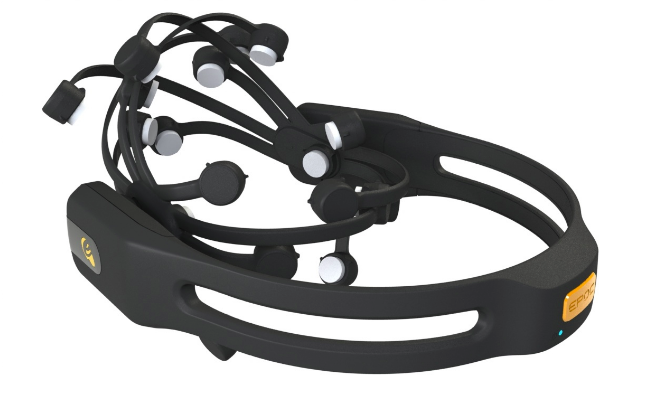
\includegraphics[scale = 0.35]{{{ImagesSSVEP/emotiv}.png}}}
    \subfigure[]{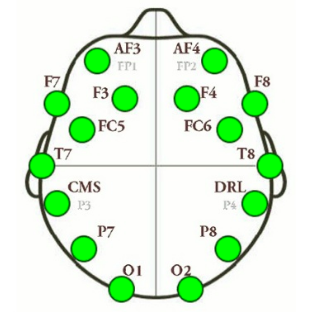
\includegraphics[width=60mm]{{{ImagesSSVEP/emotiv_elec_pos}.png}}}
    \caption{Ο ασύρματος εγκεφαλογράφος Epoc της εταιρείας Emotiv (a), και οι θέσεις που καλύπτουν τα 16 ηλεκτρόδια του, σύμφωνα με το σύστημα 10-20 (b).}
    \end{figure}
\par Επιπλέον, ενσωματωμένα μέσα στον εγκεφαλογράφο βρίσκονται τόσο αναλογικά όσο και ψηφιακά φίλτρα. Αρχικά το σήμα κάθε αισθητήρα φιλτράρεται από ένα υψηπερατό C-R φίλτρο με συχνότητα αποκοπής στα 0.16Hz, έπειτα περνάει απο ένα στάδιο προ-ενίσχυσης και στην συνέχεια απο ένα βαθυπερατό φίλτρο με συχνότητα αποκοπής 83Hz. Στο επόμενο στάδιο γίνεται δειγματοληψία του σήματος από έναν αναλογικό σε ψηφιακό μετατροπέα (ADC) με συχνότητα δειγματοληψίας 2048Hz και το σήμα φιλτράρεται από ένα ψηφιακό sinc φίλτρο 5ης τάξης για την αφαίρεση της συνιστώσας των 50Hz της τροφοδοσίας, και τέλος γίνεται υποδειγματοληψία στα 128Hz. Αν και αυτή η δειγματοληψία (128Hz) είναι ικανή για την καταγραφή συχνοτήτων ως και $64Hz$, εύρος που περιλαμβάνει την πλειοψηφία εγκεφαλικής λειτουργίας, παραμένει σημαντικά μικρότερος από τον αντίστοιχο ρυθμό δειγματοληψίας άλλων εγκεφαλογράφων αγγίζουν μέχρι και τα 2048Hz.

\par Τέλος, εκτός από τα 14 κανάλια εγκεφαλογραφήματος, η συσκευή έχει ενσωματωμένο γυροσκοπικό αισθητήρα (gyroscope), παρέχοντας 2 μετρήσεις τις γωνιακής επιτάχυνσης περί των δύο εκ των τριών αξόνων περιστροφής του κεφαλιού. Στην νεότερη εκδοχή της συσκευής, την EPOC+, παρέχονται μετρήσεις και για τον τρίτο άξονα περιστροφής, καθώς και έξι ακόμα μετρήσεις, τρείς από έναν αισθητήρα γραμμικής επιτάχυνσης (accelerometer) και τρείς από ένα μαγνητόμετρο (magnetometer).

\subsubsection{Ηλεκτρόδια}
\par Τα ηλεκτρόδια με τα οποία είναι εξοπλισμένος ο EPOC, είναι 'υγρού' τύπου, παρόλαυτα διαφέρουν αρκετά ως προς την δομή συγκριτικά με τα ευρέως χρησιμοποιούμενα Ag/Ag-Cl που αναφέρθηκαν στην παράγραφο \ref{subsec:wet_elec}
Τα συγκεκριμένα, αποτελούνται από ένα κυκλικό κομμάτι από ανοξείδωτο ατσάλι, επικαλυμμένο από μια λεπτή στρώση χρυσού. Η τελευταία στρώση αποτελείται από ένα πολυμερές υλικό υποδοχέα (polymer host) σε συνδυασμό με ένα ηλεκτρολυτικό, μη πολικό υλικό για το οποίο η εταιρεία δεν δίνει παραπάνω πληροφορίες. Η επαφή με το δέρμα γίνεται μέσω μιας κυλινδρικής τσόχας πολυεστέρα (felt pad), την οποία σε κάθε χρήση, διαποτίζουμε σε αλατούχο διάλυμα (saline) για την ελάττωσή της αντίστασης επαφής.
\par Το βασικό πρόβλημα από το οποίο υποφέρουν τα ηλεκτρόδια αυτά είναι η οξείδωση.  Παρά την λεπτή στρώση χρυσού που θα έπρεπε να την αποτρέπει, φαίνεται πως ένα απο τα άλλα υλικά της επίστρωσης, αντιδρά με το αλατούχο διάλυμα και την προκαλεί. Σύμφωνα με το τεχνικό επιτελείο της εταιρείας, δεν έχει γίνει χημική ανάλυση για να διαπιστωθεί ακριβώς η αιτία της. Τέλος, επειδή παρατηρήθηκε πως η οξείδωση ξεκινάει πάντα από την περιφέρεια του ηλεκτροδίου, είναι πολύ πιθανόν να μη είναι επαρκής η χρυσή επίστρωση σε αυτό το σημείο και να εκτίθεται το ανοξείδωτο ατσάλι στο αλατούχο διάλυμα, το οποίο αν είναι χαμηλής ποιότητας μπορεί να προκαλέσει την οξείδωση.
\par Ωστόσο η οξείδωση των ηλεκτροδίων δεν αφορά τόσο την ποιότητα του σήματος, καθώς δεν επηρεάζεται η αγωγιμότητα του ηλεκτροδίου. Το σημαντικό πρόβλημα τους αφορά την την μηχανική δομή και αντοχή τους. Παρατηρήθηκε πως μετά από το χρονικό διάστημα λίγων μηνών ξεκίνησε η φθορά στο πλαστικό σπείρωμα του πλαστικού στηρίγματος του ηλεκτροδίου, ενώ σε παλιότερα ηλεκτρόδια που υπήρχαν στο εργαστήριο, το πλαστικό στήριγμα είχε σπάσει καθιστώντας το ηλεκτρόδιο εντελώς άχρηστο. Μια αντίστοιχη παρατήρηση έγινε στην δημοσίευση \cite{Wojcik2015-pl}, όπου κατέληξαν στο συμπέρασμα πως τα ηλεκτρόδια δεν είναι ικανά να υποστηρίξουν μια έρευνα σε βάθος χρόνου, καθώς καταστρέφονται πολύ εύκολα.
\begin{figure}[H]
    \centering
    \subfigure[]{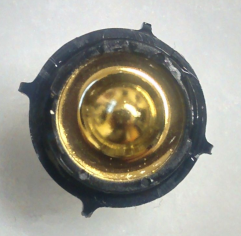
\includegraphics[width=60mm, height=40mm]{{{ImagesSSVEP/good_sensor}.png}}}
    \subfigure[]{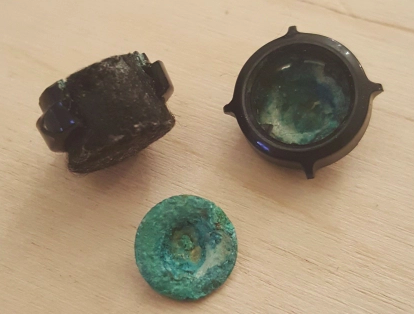
\includegraphics[width=60mm, height=40mm]{{{ImagesSSVEP/sapia_elec}.png}}}
    \subfigure[]{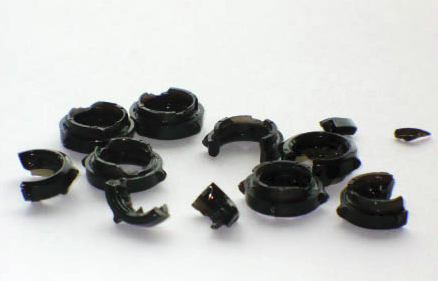
\includegraphics[width=60mm]{{{ImagesSSVEP/broken_sensors}.png}}}
    \caption{a) Καινούριο ηλεκτρόδιο χωρίς σημάδια οξείδωσης. b) Ηλεκτρόδια κατεστραμμένα από την οξείδωση, όπου πλέον δεν φαίνεται σχεδόν καθόλου η χρυσή επικάλυψη και c) Ηλεκτρόδια με σπασμένο περίβλημα έπειτα από συχνή χρήση, εικόνα από \cite{Wojcik2015-pl}.}
    \end{figure}

%\par \textcolor{red}{(Να βάλω συμβουλες για χρηση και διατηρηση ηλεκτροδίων ? )}

\subsubsection{Λογισμικό}
\textbf{Emotiv Sofware}
\par Μαζί με τον εγκεφαλογράφο Epoc, η Emotiv παρέχει μια σουίτα λογισμικού που προσφέρει στον χρήστη μια πληθώρα υπηρεσιών, άλλες δωρεάν και άλλες επί πληρωμή. 
Η βασική και δωρεάν εφαρμογή, είναι η EMOTIV Xavier Control Panel, η οποία βοηθάει τον χρήστη να κάνει την εγκατάσταση του Epoc, και να μάθει να το χρησιμοποιεί Δίνεται η δυνατότητα στον χρήστη να παρακολουθεί την ποιότητα επαφής των ηλεκτροδίων με το δέρμα αναπαριστώντας με πράσινο χρώμα την καλή ποιότητα, τις ενδιάμεσες καταστάσεις με κίτρινο και κόκκινο, ενώ μαύρο χρησιμοποιείται όταν πρακτικά λαμβάνεται μόνο θόρυβος.

\par Μια άλλη λειτουργία που παρέχεται, είναι ο υπολογισμός πέντε μετρικών εγκεφαλικής λειτουργίας σε πραγματικό χρόνο σχετικά με την συμμετοχή, την συγκέντρωση, το ενδιαφέρον, τη χαλάρωση, και το άγχος, που βιώνει ο χρήστης..

\par Τέλος παρέχεται ένα σύστημα το οποίο είναι ικανό να εκπαιδευθεί από τον κάθε χρήστη ξεχωριστά, έτσι ώστε να ξεχωρίζει συγκεκριμένες σκέψεις και να τις αντιστοιχίζει σε ξεχωριστές λειτουργίες που θα επιλέξει ο χρήστης, όπως η μετακίνηση και περιστροφή ενός εικονικού αντικειμένου ή ο έλεγχος του δείκτη του ποντικιού. Η επιτυχία αυτού του συστήματος εξαρτάται σε μεγάλο βαθμό από τον χρόνο που θα επενδύσει κάποιος στην εκπαίδευση του, καθώς και από την ικανότητα του να συγκεντρώνεται και να διαχωρίζει τις σκέψεις του. Ενδεικτικά μετά από ένα χρονικό διάστημα 10 λεπτών, επιτεύχθηκε η μετακίνηση ενός εικονικού τρισδιάστατου κύβου μπροστά και πίσω κατά βούληση, ωστόσο όταν συμπεριλήφθηκαν παραπάνω εντολές (περιστροφή δεξιόστροφη και αριστερόστροφη), τότε ήταν σχεδόν αδύνατη η μετακίνηση κύβου.
\begin{figure}[H]
    \centering
    \subfigure[]{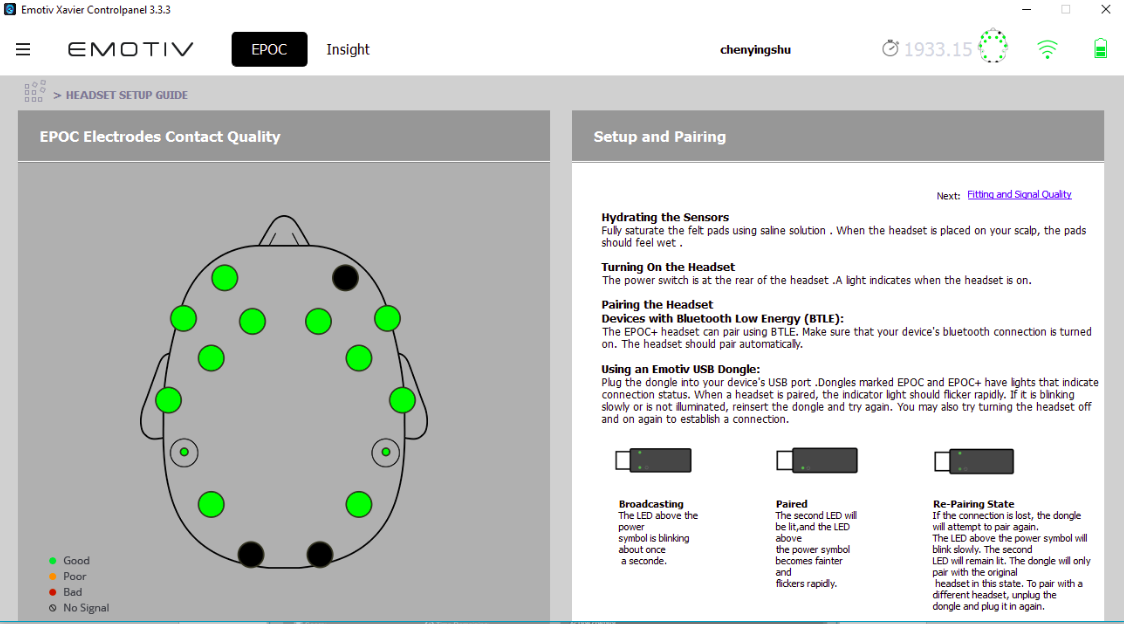
\includegraphics[width=90mm]{{{ImagesSSVEP/xavier_quality}.png}}}
    \subfigure[]{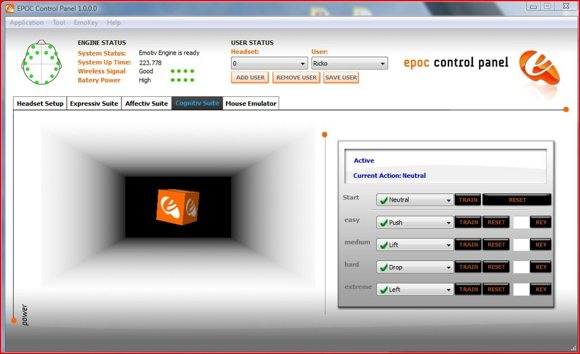
\includegraphics[width=90mm]{{{ImagesSSVEP/xavier_cube}.jpg}}}
    \caption{Το λογισμικό ελέγχου που συνοδεύει το Epoc, παρέχει ενδείξεις για την ποιότητα επαφής κάθε ηλεκτροδίου, την στάθμη της μπαταρίας καθώς και την ποιότητα της bluetooth σύνδεσης (a). Ο εικονικός κύβος που ο χρήστης μαθαίνει να ελέγχει με την σκέψη του (b). }
    \end{figure}

\textbf{Emokit}
\par Προκειμένου όμως ένας χρήστης να αποκτήσει πρόσβαση στις μετρήσεις κάθε αισθητήρα ξεχωριστά, δηλαδή στο εγκεφαλογράφημα αυτό καθ’ αυτό, θα πρέπει αγοράσει την ερευνητική έκδοση του EPOC (research Edition). Με αυτή την έκδοση, η Emotiv παρέχει το ερευνητικό κιτ ανάπτυξης λογισμικού (research SDK) το οποίο μπορεί να χρησιμοποιηθεί με μια πληθώρα προγραμματιστικών γλωσσών (C++, Python, Matlab, Java, C\#) για την επεξεργασία των εγκεφαλικών σημάτων. Το γεγονός όμως πως ο εγκεφαλογράφος που υπήρχε στο εργαστήριο δεν ήταν η ερευνητική έκδοση, μας οδήγησε στην εύρεση λύσης σε ελεύθερο λογισμικό το οποίο να παρέχει δυνατότητες παρόμοιες με αυτές του research SDK απο την Emotiv. Μια τέτοια βιβλιοθήκη είναι η Emokit και δημιουργήθηκε από την ομάδα προγραμματιστών στην OpenYou, και δίνει πρόσβαση στις μετρήσεις των αισθητήρων, την ποιότητα της επαφής και την στάθμη της μπαταρίας της συσκευής. Επιπλέον, δίνεται η δυνατότητα εξαγωγής των αποτελεσμάτων σε μορφή csv, καθώς και η αντίστροφη διαδικασία, κατά την οποία ένα csv αρχείο “διαβάζεται” σε πραγματικό χρόνο, προσομοιώνοντας τον πραγματικό εγκεφαλογράφο.

\par Στην βιβλιοθήκη συμπεριλαμβάνονται και κάποια script που υποδεικνύουν τους βασικούς τρόπους χρήσης. Αρχικά τρέχοντας το example.py εμφανίζεται ένας πίνακας με την τιμή, και την ποιότητα για κάθε ηλεκτρόδιο, τις τιμές για τον γυροσκοπικό αισθητήρα καθώς και την στάθμη της μπαταρίας.

\par Αυτού του είδους η απεικόνιση είναι μάλλον άβολη για μελέτη των εγκεφαλικών σημάτων και πιο πολύ χρησιμεύει ως ένας γρήγορος έλεγχος της ποιότητας σύνδεσης του EPOC με τον υπολογιστή.
Ένας πολύ διαφορετικό τρόπος απεικόνισης υλοποιείται στο αρχείο render.py όπου κάνοντας χρήση της βιβλιοθήκης pygame απεικονίζονται σε πραγματικό χρόνο τα διαγράμματα τιμών για κάθε ηλεκτρόδιο ξεχωριστά. Επίσης το χρώμα της γραφικής παράστασης εξαρτάται από την ποιότητα της επαφής του ηλεκτροδίου με το δέρμα. 
\begin{figure}[H]
    \centering
    \subfigure[]{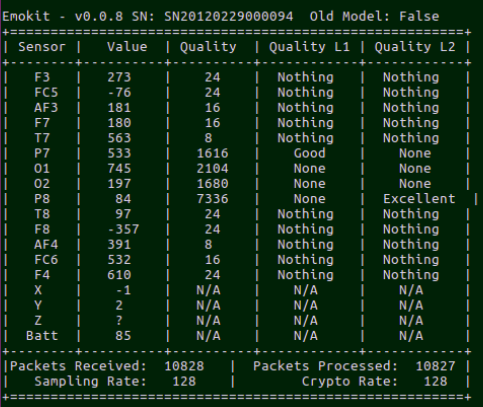
\includegraphics[width=70mm, height=60mm]{{{ImagesSSVEP/examplepy}.png}}}
    \subfigure[]{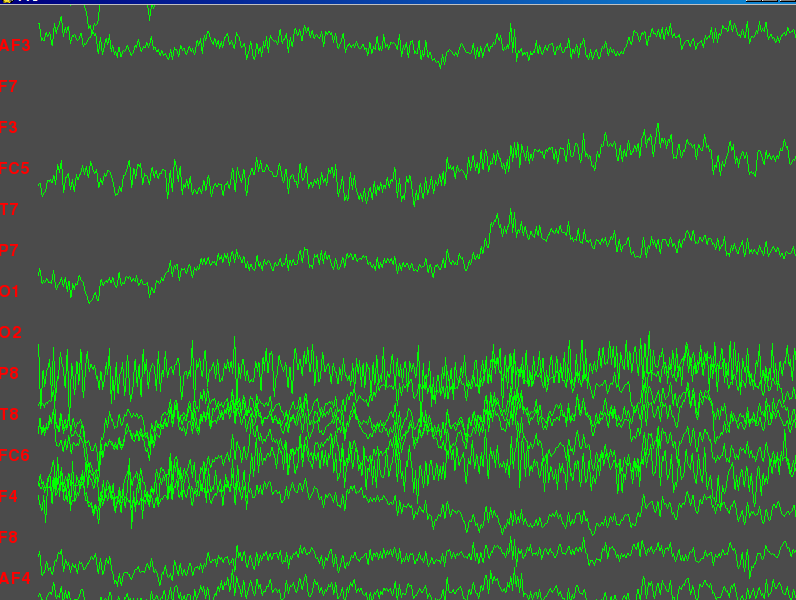
\includegraphics[width=70mm, height=60mm]{{{ImagesSSVEP/render}.png}}}
    \caption{Ο πίνακας τιμών και ποιότητας για κάθε αισθητήρα (a) και η γραφική διεπαφή οπτικοποίησης των εγκεφαλικών σημάτων (b) που παρέχονται από την βιβλιοθήκη Emokit.}
    \label{fig:render}
\end{figure}
\par Παρότι αυτού του είδους η απεικόνιση είναι πολύ χρήσιμη, ένα βασικό πρόβλημα που φαίνεται και στην εικόνα \ref{fig:render}, είναι πως τα σήματα που δίνει το EPOC περιέχουν offset, με αποτέλεσμα πολλές φορές οι γραφικές παραστάσεις να μετατοπίζονται στον κάθετο άξονα και να μπερδεύονται μεταξύ τους. Επίσης δεν παρέχεται καθόλου συχνοτική πληροφορία για κάθε κανάλι, πράγμα το οποίο θα βοηθούσε στην γρήγορη οπτικοποίηση των SSVEP σημάτων.
\par Κρίθηκε σημαντικό λοιπόν, στα πλαίσια της παρούσας διπλωματικής εργασίας, να αναπτυχθεί μια γραφική διεπαφή για την οπτικοποίηση των εγκεφαλικών σημάτων, σε Python 2.7,  με τα εξής χαρακτηριστικά :
\begin{itemize}
    \item{Χρήση του εργαλείου pyqtgraph για την δημιουργία του γραφικού περιβάλλοντος}
    \item{Ενσωμάτωση φίλτρων για την αφαίρεση του offset, και λοιπών συχνοτήτων που μπορεί να μην ενδιαφέρουν.}
    \item{Εμφάνιση του διαγράμματος Power Spectrum Density για κάθε κανάλι,  με δυνατότητα επιλογής του παραθύρου υπολογισμού του μετασχηματισμού Fourier}
    \item{Τα χρώματα των γραφικών παραστάσεων να βασίζονται στην τιμή ποιότητας για κάθε κανάλι.}
    \item{Ενδείξεις για την ακριβή τιμή της ποιότητας καθώς και για το συχνοτικό peak, στο γράφημα του χρόνου και της συχνότητας αντίστοιχα.}
\end{itemize}

\begin{figure}[H]
    \centering
    \subfigure[]{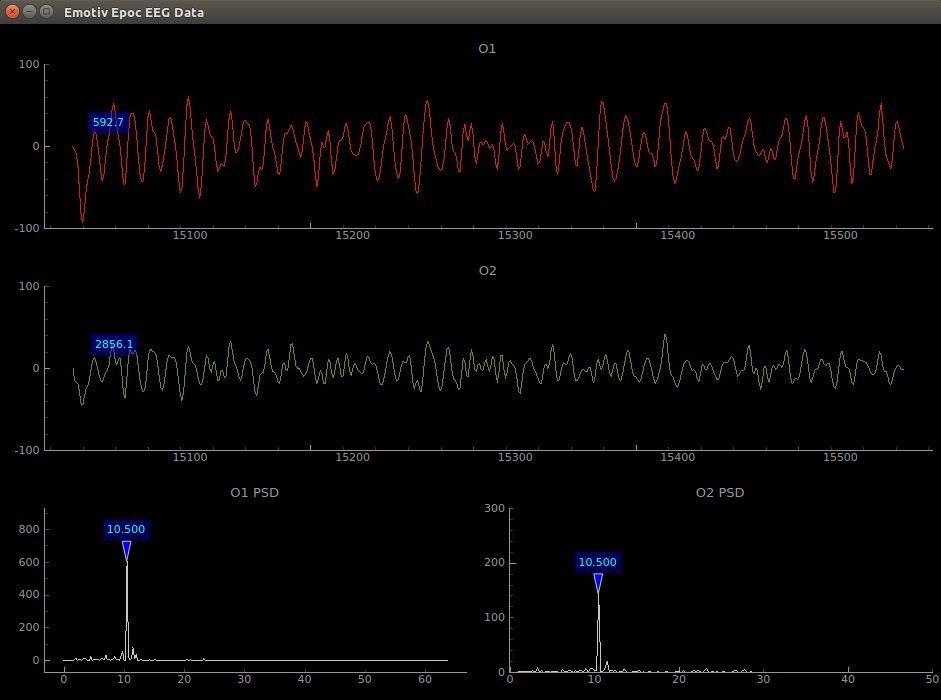
\includegraphics[width=72mm,height=50mm]{{{ImagesSSVEP/alpha_waves}.png}}}
    \subfigure[]{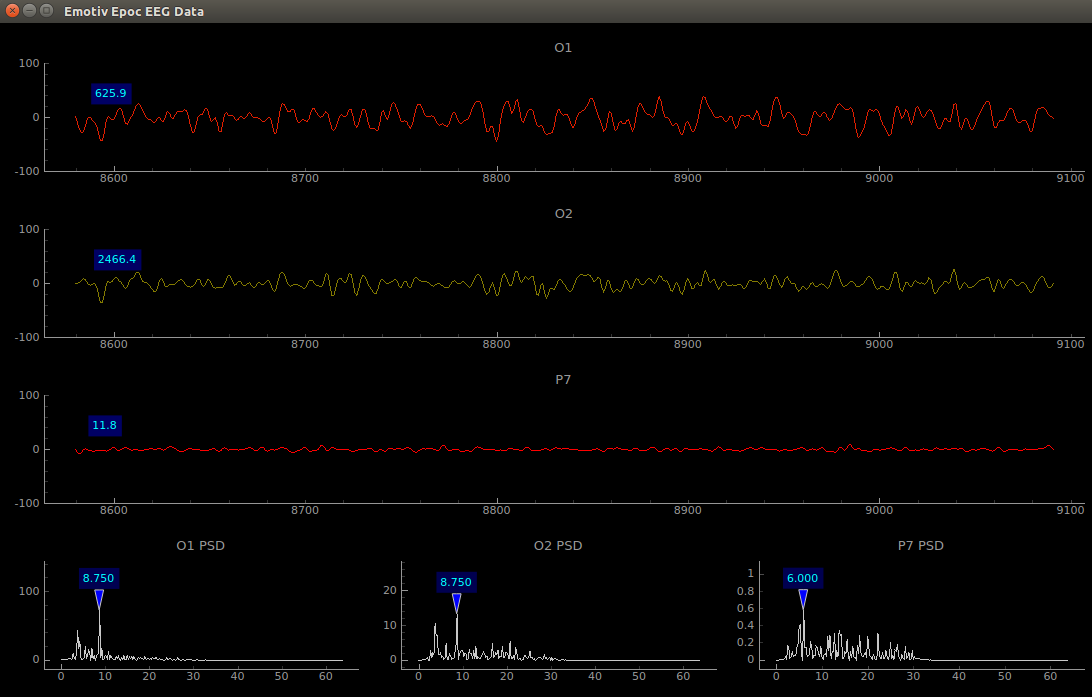
\includegraphics[width=72mm,height=50mm]{{{ImagesSSVEP/randomP7}.png}}}
    \caption{Η γραφική διεπαφή που υλοποιήσαμε για την οπτικοποίηση επιλεγμένων καναλιών στο πεδίο του χρόνου και της συχνότητας. Στην αριστερή εικόνα o χρήστης είχε κλειστά μάτια και επιλέχθηκαν τα κανάλια Ο1 και Ο2 οπού φαίνονται ξεκάθαρα τα άλφα κύματα στα $10.5Hz$, ενώ στην δεξιά εικόνα ο χρήστης άνοιξε τα μάτια του, και  προστέθηκε και το κανάλι P7.}
    \label{fig:epoc_gui}
\end{figure}

\subsection{Υπολογιστής}
\par Η όλη εφαρμογή υλοποιήθηκε σε έναν φορητό υπολογιστή ASUS με επεξεργαστή Intel Pentium i7 και χρησιμοποιώντας το λειτουργικό σύστημα Ubuntu. Παρότι η βιβλιοθήκη Emokit υποστηρίζεται τόσο για Windows όσο και για Unix λειτουργικά, διάφορα προβλήματα που παρουσιάστηκαν στην επικοινωνία του EPOC με τον υπολογιστή στο Windows περιβάλλον, ώθησαν στην επιλογή του Ubuntu.

\subsection{Συστοιχίες LED}
\par Στην υποενότητα \ref{subsec:visual_stimulus} αναλύθηκαν οι πιο συχνοί τρόποι που χρησιμοποιούνται για την επίτευξη της επαναλαμβανόμενης οπτικής διέγερσης (ΕΟΔ), καθώς και τα χαρακτηριστικά της καθεμιάς. Σστην παρούσα εργασία επιλέχθηκε η μέθοδος των LEDs, καθώς οι διεπαφές που τα χρησιμοποιούν ως ΕΟΔ, επιτυγχάνουν κατά μέσο όρο υψηλότερες επιδόσεις accuracy, και ITR \cite{zhu2010survey}. Σε αυτήν την υπόενότητα θα γίνει μια παρουσίαση των LED συστοιχιών που κατασκευάστηκαν καθώς και της βάσης τους η οποία προσαρμόζεται στην οθόνη ενός φορητού υπολογιστή.

\subsubsection{Επιλογή χρώματος LED}
\par Ένας από τα βασικά χαρακτηριστικά των LED, που παίζει σημαντικό ρόλο στην ποιότητα των SSVEP σημάτων που θα προκληθούν στον εγκέφαλο, είναι το χρώμα των LED \cite{zhu2010survey}. Αποτελεί άλλη μια από τις παραμέτρους αυτών των διεπαφών που δεν έχουν μελετηθεί αρκετά έτσι ώστε να βρεθεί μια κοινή αποδεκτή επιλογή χρώματος. Είναι γεγονός βέβαια πως η βέλτιστη επιλογή ίσως διαφέρει σημαντικά από χρήστη σε χρήστη λόγω των αποκλίσεων μεταξύ τους όσον αφορά την φυσιολογία του οφθαλμού. 

\par Το μάτι αποτελείται από τριών ειδών φωτο-υποδοχείς που είναι ευαίσθητοι στο κόκκινο, μπλε και πράσινο χρώμα αντίστοιχα. Σύμφωνα με την έρευνα του W. D. Wright \cite{Gregory1978-lj}, καθένας από αυτούς ανταποκρίνεται στο χρώμα που έχει ευαισθησία, με τον φωτο-υποδοχέα που είναι ευαίσθητος στο κόκκινο χρώμα, να παράγει τα πιο δυνατά σήματα. Συνεπώς μπορούμε αν υποθέσουμε πως τα LED κόκκινου χρώματος προκαλούν τα ισχυρότερα SSVEP σήματα. Μια άλλη σκέψη είναι πως η οπτική διέγερση άσπρου φωτός θα παράγει ακόμα ισχυρότερα σήματα, καθώς το άσπρο φως είναι ικανό να διεγείρει όλους τους φωτο-υποδοχείς ταυτόχρονα. Η πλειοψηφία των ερευνών σε αυτόν το τομέα φαίνεται να επιβεβαιώνει τις παραπάνω παρατηρήσεις. Στις δημοσιεύσεις \cite{Bieger2010-bv,Cao2012-yb} κατέληξαν πως το άσπρο χρώμα επιτυγχάνει υψηλότερο ITR, ενώ στην \cite{2015-of}, κατέληξαν στο κόκκινο, χωρίς όμως να δοκιμάσουν το άσπρο. Αντιθέτως στις \cite{Singla2013-pd} επιλέχθηκε το μοβ, ενώ στην \cite{Chu2017-uk} κατέληξαν πως το μοβ παράγει τα λιγότερο ισχυρά SSVEP. Τέλος στην \cite{zhu2010survey} παρατήρησαν πως από όλες τις 58 δημοσιεύσεις που μελέτησαν, υψηλότερο ITR επιτευχθεί με την χρήση πράσινων LED. 

\par Ορμώμενοι από τις παραπάνω παρατηρήσεις, και θέλοντας να μεγιστοποιήσουμε τις πιθανότητες να παραχθούν ισχυρά SSVEPs, κατασκευάσαμε δοκιμαστικά μια συστοιχία LEDs άσπρου χρώματος και μία πράσινου. Παρότι τα άσπρου χρώματος LED φαίνεται να αποδίδουν καλύτερα, σε δοκιμές που κάναμε χρησιμοποιώντας μια συστοιχία 25 LEDs, διατεταγμένα 5x5,  παρατηρήθηκε πολύ έντονη κόπωση των ματιών σε όλα τα άτομα που δοκίμασαν να κοιτάξουν τα LED. Συγκεκριμένα, ήταν αδύνατο να κρατήσουν οπτική επαφή για πάνω από 1 λεπτό, συνεπώς ενώ τα άσπρα LED παρήγαγαν πολύ δυνατά SSVEP σήματα σε όλα τα άτομα, έπρεπε να επιλεχθούν LED διαφορετικού χρώματος.
%ΕΙΚΟΝΑ ΑΠΟ SSVEP WHITE LEDS ?? σε συγκριση και με τα πρασινα ?? φτιαξε ενα πειραμα.
Έπειτα από δοκιμές με κόκκινα και πράσινα LED, παρατηρήθηκε πολύ μικρή διαφορά στα μεταξύ τους παραγόμενα SSVEP σήματα, συνεπώς καταλήξαμε στα πράσινα όντας τα πιο ξεκούραστα για το μάτι, ακόμα και σε πολύ δυνατές φωτεινές εντάσεις, συμπέρασμα στο οποίο κατέληξαν και στις \cite{2015-of,zhu2010survey,Bieger2010-bv}

\par Τα LED που επιλέχθηκαν έπρεπε να ικανοποιούν δύο βασικές προϋποθέσεις: 
\begin{itemize}
    \item{Nα έχουν πολύ καλή απόδοση, έτσι ώστε να πετύχουμε υψηλή φωτεινότητα με το ελάχιστο ρεύμα οδήγησης}
    \item{Nα έχουν ευρεία γωνία θέασης, καθώς στην αντίθετη περίπτωση, οι συστοιχίες που δεν βρίσκονται σε ευθυγράμμιση με το μάτι, δεν θα είναι ικανές να παράγουν τόσο δυνατά SSVEPs, όσο αυτές που θα βρίσκονται ακριβώς απέναντι από τον χρήστη. }
\end{itemize} 
\par Τα LED που επιλέχθηκαν κατασκευάζονται από την εταιρεία YETDA, με κωδικό SSOOTGlD-H, μήκος κύματος εκπεμπόμενου φωτός στα $525nm$ και γωνία θέασης τις $80^{\circ}$.

\subsubsection{Κατασκευή συστοιχιών}
\par Στην συγκεκριμένη διεπαφή θα χρησιμοποιήσουμε 4 επαναλαμβανόμενες οπτικές διεγέρσεις (ΕΟΔ) οπού η κάθε μία θα ταλαντώνεται διαφορετική συχνότητα, συνεπώς θα χρειαστούν 4 συστοιχίες LED. Ο αριθμός των LED για κάθε συστοιχία επιλέχθηκε να είναι 20, σε διάταξη 5x4. Επιλέχθηκε μεγάλος αριθμός έτσι ώστε επηρεάζοντας την τροφοδοσία των led, να υπάρχει δυνατότητα πειραματισμού με την ένταση του φωτισμού, η οποία μπορεί να κυμαίνεται από αμυδρό φωτισμό των led, μέχρι πολύ δυνατή ένταση που κουράζει γρήγορα τα μάτια. Επιπλέον, σε κάθε συστοιχία προστέθηκε ένα επιπρόσθετο κόκκινο LED διαμέτρου 3mm, του οποίου η χρησιμότητα είναι διττή. Κατά την διάρκεια της offline ανάλυσης των σημάτων θα σηματοδοτεί ποια συστοιχία θα πρέπει να κοιτάξει ο χρήστης (cue mechanism), ενώ κατά την διάρκεια της online χρήσης της διεπαφής, θα έχει τον ρόλο της ανάδρασης ενημερώνοντας τον χρήστη για την έξοδο της διεπαφής (feedback mechanism). Κάθε συστοιχία υλοποιήθηκε πάνω σε ένα stripboard όπου καθένα από αυτά θα ενσωματώνεται σε μια ξύλινη βάση που μπορεί να προσαρμόζεται σε κάθε είδους λεπτή οθόνη.

\begin{figure}[H]
    \centering     %%% not \center
    \subfigure[]{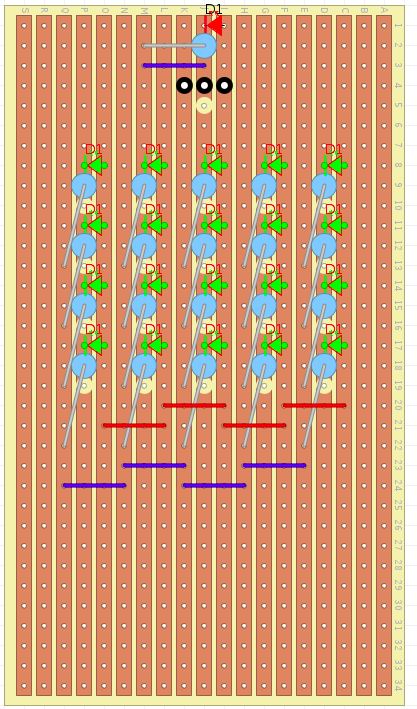
\includegraphics[width=40mm,height=60mm]{{{ImagesSSVEP/led_vero}.png}}}
    \subfigure[]{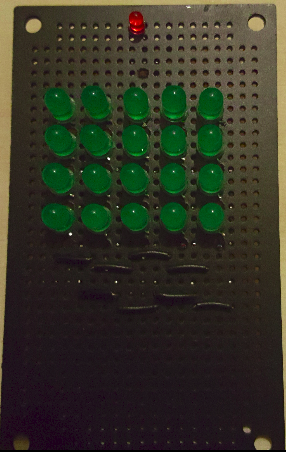
\includegraphics[width=40mm,height=60mm]{{{ImagesSSVEP/led_front2}.png}}}
    \subfigure[]{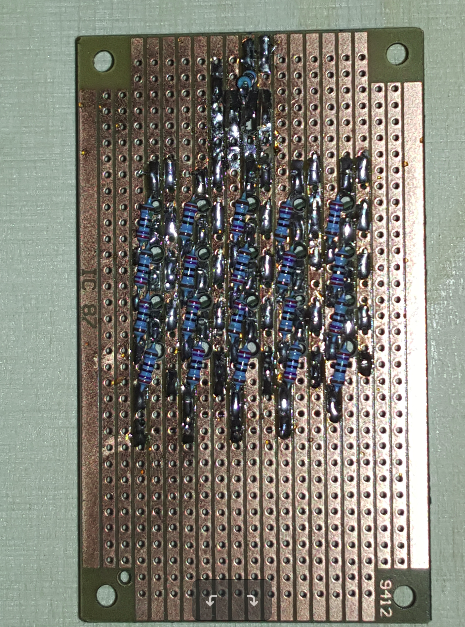
\includegraphics[width=40mm,height=60mm]{{{ImagesSSVEP/led_back}.png}}}
    \subfigure[]{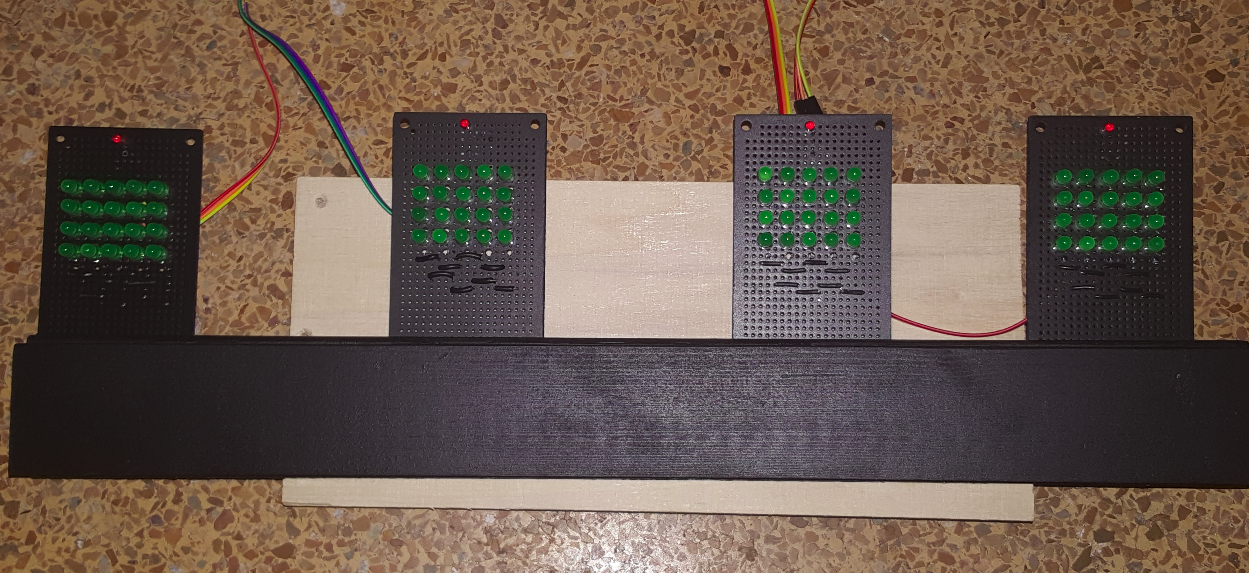
\includegraphics[scale=0.2]{{{ImagesSSVEP/all_LED_front}.png}}}
    \caption{Η μια από τις τέσσερις LED συστοιχίες που υλοποιήσαμε, a) ο φυσικός σχεδιασμός της σε stripboard (b) η μπροστινή και (c) και πίσω όψη. d) και οι τέσσερις συστοιχίες τοποθετημένες στην ξύλινη βάση.}
    \label{fig:driver_circuit}
\end{figure}


\subsubsection{Κύκλωμα Οδήγησης}
\par Για τις απαιτήσεις του πειράματος απαιτούνταν ο πλήρης έλεγχος των LED, δηλαδή η δυνατότητα ξεχωριστών σημάτων ελέγχου για κάθε μια από τις 4 συστοιχίες, καθώς και για τα 4 κόκκινα LEDs συνεπώς χρειάζεται ένας μικρο-ελεγκτής με τουλάχιστον 8 ψηφιακές εξόδους, καθώς και να είναι πολύ μικρός σε μέγεθος έτσι ώστε να ενσωματωθεί εύκολα στην συνολική πλακέτα οδήγησης. Τελικώς, χρησιμοποιήθηκε ο μικροελεγκτής Arduino Nano, που παρέχει 22 ψηφιακές θύρες εισόδου/εξόδου καθώς και ειδικούς ακροδέκτες που καθιστούν εύκολη την εφαρμογή του σε πλακέτες.  
\par Κάθε συστοιχία αποτελείται από 20 LEDs και κάθε LED χρειάζεται περίπου $3mA$ για να παράγει επαρκή φωτεινότητα για τις απαιτήσεις του πειράματος, συνεπώς το ρεύμα που απαιτείται για την οδήγηση κάθε συστοιχίας είναι περίπου $60mA$, το οποίο ξεπερνάει το μέγιστο ρεύμα που μπορεί να διαχειριστεί κάθε έξοδος του Arduino ($40mA$). Συνεπώς χρησιμοποιήθηκαν 8 τρανζίστορ, ένα για κάθε συστοιχία και ένα για κάθε κόκκινο LED. Το κύκλωμα μπορεί να τροφοδοτηθεί είτε από την θύρα Vin του arduino, που ταυτίζεται  με την  έξοδο των $5volt$ της θύρας USB στην οποία συνδέεται, είτε από εξωτερική DC τροφοδοσία, καθώς στο κύκλωμα περιλαμβάνεται o σταθεροποιητής τάσης LM317.

\begin{figure}[H]
    \centering     %%% not \center
    \subfigure[]{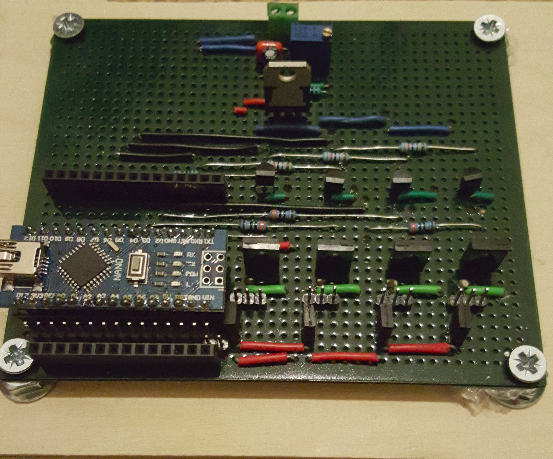
\includegraphics[width=60mm,height=50mm]{{{ImagesSSVEP/driver_circuit}.png}}}
    \caption{To κύκλωμα οδήγησης των LED. Ένα arduino Nano δίνει τα σήματα ελέγχου σε καθένα απο τα 8 τρανζίστορ για τον έλεγχο 4 LED συστοιχιών και 4 ενδεικτικών κόκκινων LED. }
    \label{fig:driver_led}
\end{figure}
 
\subsubsection{Λογισμικό Arduino}
\par Όπως έχει αναφερθεί, ο σκοπός που πρέπει να επιτευχθεί είναι κάθε συστοιχία να αναβοσβήνει με την δικής της συχνότητα ανεξάρτητα από τις άλλες. Είναι σημαντικό να υπάρχει απόλυτη ακρίβεια στην συχνότητα, και ευκολία στην επιλογή της κάθε μίας, για να διευκολυνθεί η διαδικασία των πειραματισμών. Προς την ίδια κατεύθυνση θέλουμε να υπάρχει και η δυνατότητα επιλογής διαφορετικού duty cycle για κάθε συστοιχία καθώς,  όπως θα φανεί και στην συνέχεια, επηρεάζει την ποιότητα των SSVEP σημάτων. Ενώ είναι πολύ εύκολο να επιτευχθεί η δημιουργία τετραγωνικού παλμού σε μια ψηφιακή έξοδο του Arduino, πχ ρυθμίζοντας ακριβώς τον χρόνο που θα είναι On και Off με την χρήση της εντολής delay(), η επέκταση αυτής της λειτουργίας και σε άλλες εξόδους ταυτόχρονα απαιτεί την χρήση την χρήση ενός thread για κάθε διαφορετική έξοδο, τα οποία να εργάζονται παράλληλα. Για αυτό το λόγο χρησιμοποιήθηκε η βιβλιοθήκη Timer του Simon Monk η οποία επιτελεί αυτόν ακριβώς τον σκοπό. Παρόλαυτά δεν παρέχεται η δυνατότητα επιλογής duty cycle, το οποίο παραμένει σταθερά στο $50\%$. Για τον λόγο αυτό τροποποιήθηκε o πυρήνας της βιβλιοθήκης έτσι ώστε ο χρήστης να μπορεί να θέσει ακριβώς την διάρκεια On και Off του παλμού.\\\\

\lstinputlisting[caption=\text{Παράδειγμα χρήσης της τροποποιημένης timer.h, για την δημιουργία παλμών μεταβλητού duty cycle}, language=C]{Code/blink_timer.ino}

\par Τέλος, επειδή η κατάσταση  των LED πρέπει να ελέγχεται πλήρως από την διεπαφή, η οποία θα είναι γραμμένη σε  Python, χρησιμοποιήθηκε η βιβλιοθήκη Pyserial, έτσι ώστε η διεπαφή και το Arduino να επικοινωνούν σειριακά μέσω της USB θύρας. Με αυτό τον τρόπο είναι δυνατός ο έλεγχος της εκκίνησης η της παύσης των LEDs, καθώς και των κόκκινων ενδεικτικών LEDs.

\begin{figure}[H]
    \centering     %%% not \center
    \subfigure[]{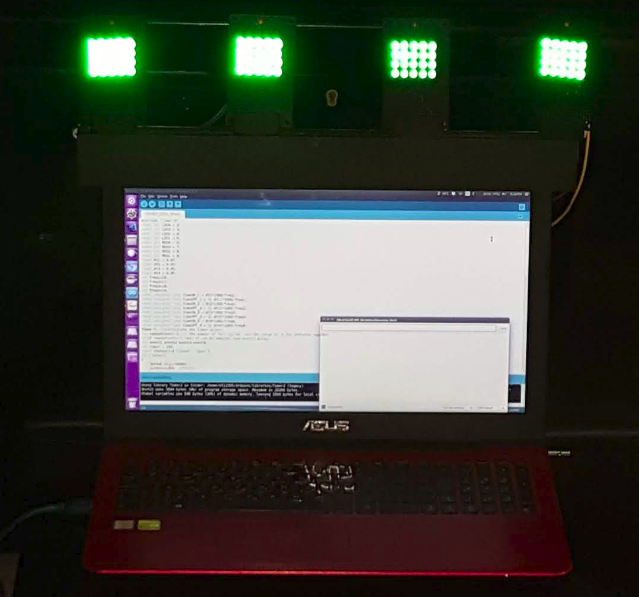
\includegraphics[width=60mm,height=50mm]{{{ImagesSSVEP/base_on_laptop}.jpg}}}
    \subfigure[]{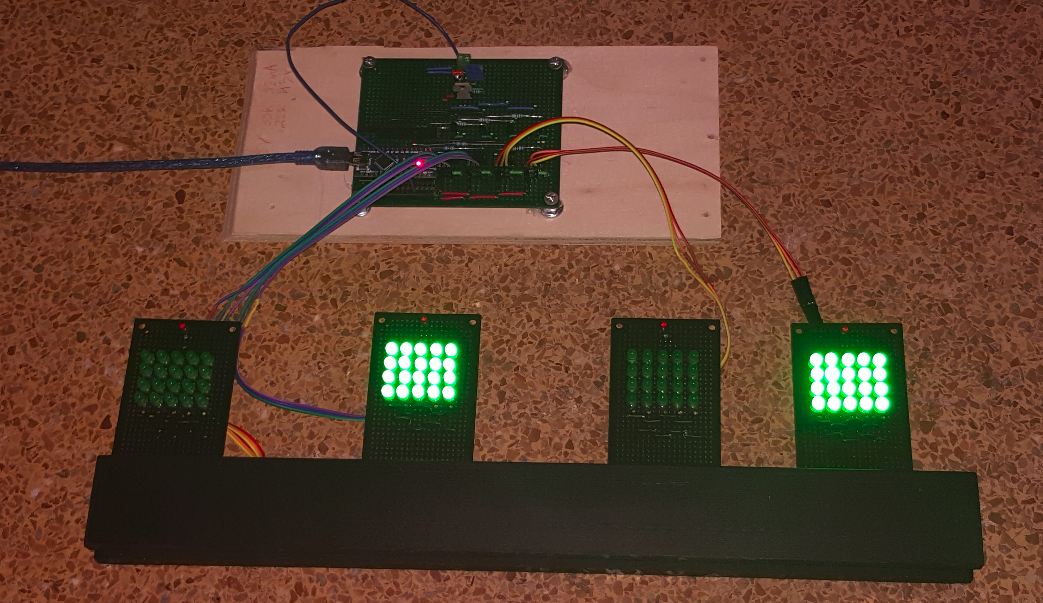
\includegraphics[width=60mm,height=50mm]{{{ImagesSSVEP/on_the_floor}.png}}}
    \caption{Η ολοκληρωμένη διάταξη με την βάση, τις συστοιχίες και το κύκλωμα οδήγησης εν ώρα λειτουργίας. }
    \label{fig:base_leds_working}
\end{figure}

\section{Offline Καταγραφή των Σημάτων}
\subsection{Περιγραφή Συστήματος}
\par Προκειμένου να υλοποιηθεί μια διεπαφή η οποία θα ανιχνεύει και θα αποκωδικοποιεί επιτυχώς τα  SSVEP σήματα, σε πραγματικό χρόνο, θα πρέπει πρώτα να γίνει σχολαστική offline μελέτη των σημάτων καθώς και εκπαίδευση του συστήματος απόφασης.
\begin{figure}[H]
    \centering     
    \subfigure[]{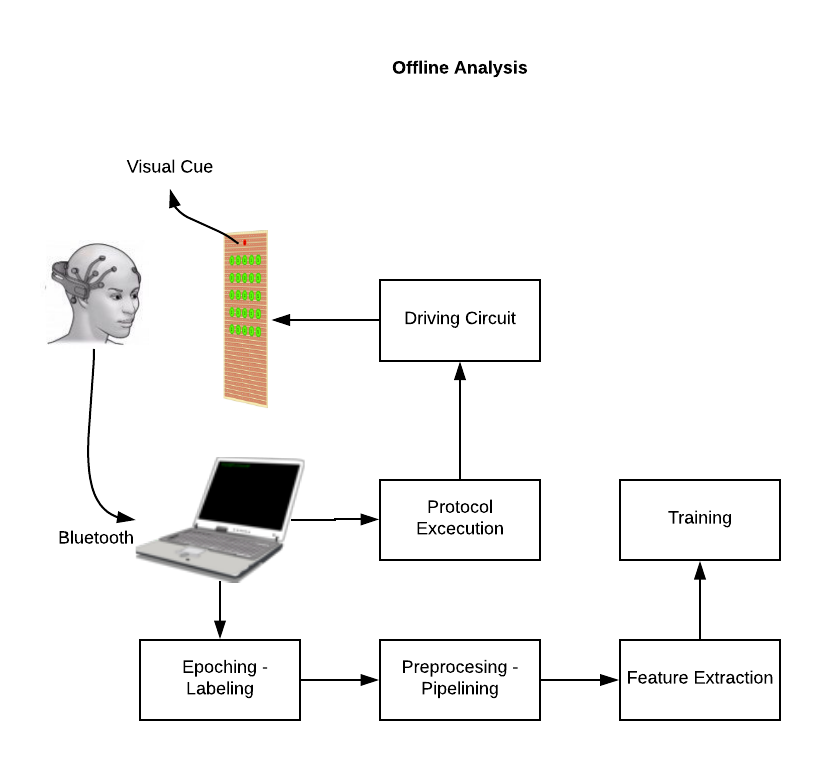
\includegraphics[scale=0.35]{{{ImagesSSVEP/offline_analysis}.png}}}
    \caption{Διάγραμμα που παρουσιάζει τα στάδια του offline συστήματος καταγραφής δεδομένων.}
    \label{fig:offline_analysis}
\end{figure}

\par Ο χρήστης πρέπει να κοιτάξει προς την συστοιχία της οποίας το κόκκινο LED ανάβει κάθε φορά. Με αυτόν τον τρόπο το πρόγραμμα γνωρίζει ποια ΕΟΔ κοιτούσε ο χρήστης κάθε χρονική στιγμή. Το επόμενο στάδιο περιλαμβάνει την διαδικασία της κατάτμησης του συνολικού σήματος στα χρονικά σημεία οπού το πρόγραμμα έδινε εντολή στον χρήστη να στρέψει το βλέμμα του σε διαφορετική συστοιχία, διαδικασία γνωστή ως epoching. Στην συνέχεια υπάρχει το στάδιο της προ-επεξεργασίας των δεδομένων, κατά το οποίο εφαρμόζονται οι διάφορες τεχνικές αποθορυβοποίησης. Επόμενο βήμα είναι η εξαγωγή αντιπροσωπευτικών χαρακτηριστικών από το σήμα, τα οποία θα χρησιμοποιηθούν για το τελευταίο στάδιο της εκπαίδευσης του συστήματος απόφασης. Καθένα από τα προαναφερθέντα στάδια θα αναλυθεί διεξοδικά στην συνέχεια.

\subsection{Πειραματική διάταξη}
\label{subsec:experimental_setup}
\par Η καταγραφή των δεδομένων έγινε σε 2 άτομα ηλικίας 20 και 25 ετών, χωρίς προηγούμενο ιατρικό ιστορικό σχετικά με οφθαλμικές παθήσεις ή επεισόδια επιληψίας, καθώς όπως αναφέρθηκε και στην υποενότητα \ref{subsec:visual_stimulus} η έκθεση σε απότομες εναλλαγές φωτός στην χαμηλή συχνοτική περιοχή, είναι ικανή να προκαλέσει επιληπτικές κρίσεις σε ευαίσθητα άτομα, ενώ προηγούμενες οφθαλμικές παθήσεις, ίσως να επηρεάζουν την ποιότητα των SSVEP σημάτων.

\par Η χρωματική αντίθεση (color contrast) μεταξύ των 2 καταστάσεων  on και off κάθε πηγής φωτός, φαίνεται να παίζει σημαντικό ρόλο στην ποιότητα των παραγόμενων σημάτων. Δυο είναι οι τρόποι για την επίτευξη υψηλής αντίθεσης, α) η αύξηση της φωτεινότητας των LED και β) η μείωση του φωτός από το δωμάτιο στο οποίο πραγματοποιείται το πείραμα. Σε αυτή την κατεύθυνση λοιπόν, όλα τα πειράματα πραγματοποιήθηκαν σε σχεδόν σκοτεινό δωμάτιο, τακτική η οποία φαίνεται να ακολουθείται αρκετά συχνά \cite{Allison2010-mg}. Πιο συγκεκριμένα, ακολουθεί ένας πίνακας μετρήσεων φωτεινότητας σε LUX για όλες τις φωτεινές καταστάσεις κατά την διάρκεια της καταγραφής.

\begin{table}[H]
	\centering
    \begin{tabular}{| l | l | l | l |}
    \hline
    \textbf{LEDs / RoomLight} & \textbf{ON} & \textbf{OFF}\\ \hline
    ON  & NaN & NaN \\ \hline
    OFF & NaN & NaN \\ \hline
    \hline
    \end{tabular}
	\caption{Μετρήσεις όλων των καταστάσεων φωτεινότητας κατά την διάρκεια της καταγραφής δεδομένων.}
	\label{tab:lux}
\end{table}
% https://www.researchgate.net/figure/Functional-model-of-an-SSVEP-based-BCI_fig1_264999108

\subsection{Πρωτόκολλο Καταγραφής Δεδομένων}
\subsubsection{Περιγραφή}
\label{subsec:protocol}
\par Απαραίτητη προϋπόθεση για αυτήν την μελέτη είναι η δημιουργία ενός πρωτοκόλλου καταγραφής των δεδομένων, το οποίο θα ακολουθείται πιστά σε κάθε καταγραφή για κάθε άτομο, έτσι ώστε να υπάρχει συνέπεια μεταξύ όλων των πειραματικών δοκιμών, πράγμα το οποίο επιτρέπει την ασφαλή σύγκριση αποτελεσμάτων και εξαγωγή συμπερασμάτων.

\begin{figure}[H]
    \centering     
    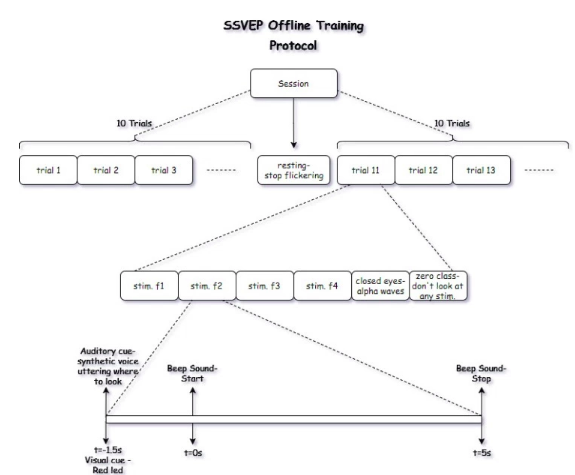
\includegraphics[scale=0.5]{{{ImagesSSVEP/protocol}.jpg}}
    \caption{Διάγραμμα που απεικονίζει την διαδικασία που ακολουθείται για την καταγραφή των δεδομένων, σύμφωνα με ένα πρωτόκολλο που σχεδιάστηκε για αυτή την εργασία}
    \label{fig:protocol}
\end{figure}

\par Όπως φαίνεται, κάθε πειραματική περίοδος (session) αποτελείται από 20 δοκιμές (trials) με μια ενδιάμεση περίοδο ξεκούρασης κατά την οποία κλείνουν όλες οι LED συστοιχίες. Σε κάθε δοκιμή ο υποδεικνύεται στον χρήστη να εκτελέσει έξι εντολές. Οι τέσσερις από αυτές αντιστοιχούν στην στρέψη του βλέμματος σε κάθε μια από τις τέσσερις διαφορετικές LED συστοιχίες, ενώ στις υπόλοιπες δύο, ο χρήστης ζητείται να κλείσει τα μάτια του (alpha waves) και τέλος να μην παρατηρεί καμία από τις τέσσερις συστοιχίες (No-Control). Ο ρόλος των δύο τελευταίων θα φανεί στην παράγραφο \ref{sec:online_design}, όπου θα γίνει ο σχεδιασμός του online σκέλους της διεπαφής. Μια σημαντική παρατήρηση είναι πως η σειρά αυτών των εντολών υπαγορεύεται στον χρήστη με τυχαία σειρά για κάθε δοκιμή, λεπτομέρεια που συχνά παραβλέπεται από αντίστοιχες έρευνες. Η τυχαία σειρά των εντολών προσομοιώνει καλύτερα καταστάσεις πραγματικού χρόνου, οπού δεν υπάρχει πάντα συσχέτιση μεταξύ μιας εντολής και της επόμενης που θα ακολουθήσει. Επιπλέον κάθε μια από τις εντολές υποδεικνύεται στον χρήστη με δύο τρόπους: α) Ακουστικό σήμα, οπού μια συνθετική φωνή ανακοινώνει το νούμερο της εντολής (one, two, three, four) και β) Οπτικό σήμα, που υλοποιείται από το κόκκινο LED που βρίσκεται στην κορυφή κάθε συστοιχίας. Τέλος δύο ακόμα ακουστικά ερεθίσματα παράγονται μετά την προηγούμενη υπόδειξη, τα οποία σηματοδοτούν την έναρξη και την λήξη της δοκιμής. Μεταξύ της αρχικής υπόδειξης και της πραγματικής έναρξης της δοκιμής παρεμβάλλεται 1.5 δευτερόλεπτο , και ο λόγος είναι πως ο χρήστης χρειάζεται λίγο χρόνο για να στρέψει το βλέμμα του μεταξύ δύο διαφορετικών συστοιχιών.

\par Μια σημαντική παράμετρος που έπρεπε να ρυθμιστεί είναι η διάρκεια της κάθε δοκιμής (trial). Η διάρκεια αυτή συμπίπτει με την διάρκεια του κάθε epoch που θα δημιουργηθεί στην συνέχεια. Ο σκοπός είναι να πειραματιστούμε με διάφορα μεγέθη epoch, έτσι ώστε να αποφανθούμε γι αυτό που δίνει τα καλύτερα αποτελέσματα . Η βέλτιστη διάρκεια που θα προκύψει, θα καθορίσει και χρονικό παράθυρο στο οποίο θα αναλύονται τα SSVEP σήματα στην real time-online εκδοχή της διεπαφής, δηλαδή το ελάχιστο χρονικό διάστημα μεταξύ δυο διαδοχικών αποφάσεων. Παρότι η επεξεργασία χρονικών παραθύρων μεγάλων σε διάρκεια (π.χ 10 δευτερόλεπτα) είναι πιθανόν να επιφέρει καλύτερα ποσοστά ταξινόμησης, μια διεπαφή τέτοιου είδους, που παίρνει αποφάσεις με τέτοια καθυστέρηση είναι πρακτικά άχρηστη. Συνεπώς καταλήξαμε πως η μέγιστη χρονική διάρκεια που αξίζει να μελετήσουμε είναι τα 5 sec. 

\subsubsection{Λογισμικό}

\par Το πρωτόκολλο αυτό υλοποιήθηκε σε γλώσσα Python. Η δημιουργία ενός προγράμματος που θα υλοποιεί αυτή την περίπλοκη διαδικασία καταγραφής των δεδομένων ήταν απαραίτητη για διάφορους λόγους και συνέβαλε στην αυτοματοποίηση της όλης διαδικασίας. 
\par Αρχικά πρέπει να αναφερθεί πως όση ώρα κρατάει η διαδικασία, τα δεδομένα καταγράφονται συνεχώς από το EPOC, χωρίς δηλαδή να υπάρχει διακοπή κάθε φορά που το πρόγραμμα υπαγορεύει στον χρήστη μια καινούρια εντολή. Συνεπώς παράλληλα με την καταγραφή των δεδομένων, καταγράφονται και οι χρονικές στιγμές στις οποίες υπαγορεύονται οι εντολές σε ένα log αρχείο, έτσι ώστε στην συνέχεια, να μπορούν να δημιουργηθούν τα epochs και τα labels τους, κάνοντας κατάτμηση της συνολικής καταγραφής σε αυτές τις χρονικές στιγμές. 
\par Επίσης ένα σημαντικό χαρακτηριστικό του προγράμματος, είναι η ικανότητα οργανώνει τις καταγραφές σε διαφορετικούς φακέλους αναλόγως την πειραματική συνεδρία (session) και τον χρήστη. Κάθε φορά, στην αρχή του session, ο χρήστης δηλώνει το όνομά του, και το πρόγραμμα δημιουργεί έναν φάκελο με όνομα της μορφής “Id\_UserName”. Στην συνέχεια δίνει ένα όνομα για το session, και δημιουργείται ο φάκελος με όνομα της μορφής “SessionName\_Timestamp” στον οποίο θα αποθηκευτούν όλα τα αρχεία που αφορούν την συγκεκριμένη καταγραφή. Επιπλέον, προαιρετικά, ο χρήστης μπορεί να προσθέσει κάποια σχόλια που αφορούν την συγκεκριμένη καταγραφή. Για παράδειγμα την κατάσταση του φωτισμού στο δωμάτιο (ανοιχτά ή κλειστά φώτα, μετρήσεις LUX), τα χαρακτηριστικά της φωτεινής πηγής (χρώμα LED, ένταση κλπ), την απόσταση από τα LED, καθώς και σχόλια για την κατάσταση του ίδιου του ατόμου όπως ώρες ύπνου, επίπεδα κούρασης ή ακόμα και την πληροφορία για την πυκνότητα των μαλλιών του την στιγμή της καταγραφής. Όλες αυτές παράμετροι επηρεάζουν σημαντικά την ποιότητα των παραγόμενων σημάτων, και συνεπώς είναι σημαντικό να καταγραφούν ως meta-data, καθώς θα βοηθήσουν και στην επιλογή των βέλτιστων συνθηκών καταγραφής. Τέλος για κάθε session, αποθηκεύονται σε μία κλάση SessionInfo, όλες εκείνες οι μεταβλητές που είναι απαραίτητες για την offline ανάλυση των δεδομένων, όπως η συχνότητες διέγερση, η διάρκεια κάθε trial κ.α

\begin{figure}[H]
    \centering     %%% not \center
    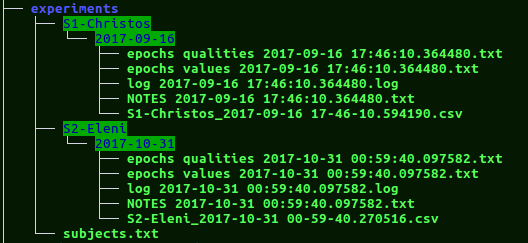
\includegraphics[scale=0.7]{{{ImagesSSVEP/dir_tree}.png}}
    \caption{Η οργάνωση των καταγραφών για κάθε χρήστη και κάθε συνεδρία.}
    \label{fig:dir_tree}
\end{figure}

\subsection{Προεπεξεργασία δεδομένων}
\label{subsec:preprocessing}

\subsubsection{Epoching}

\par Προκειμένου να γίνει η εύκολη επεξεργασία των δεδομένων, είναι απαραίτητη η κατάτμηση του συνολικού εγκεφαλογραφήματος, σε τέτοια σημεία που να οριοθετούν κάθε trial για κάθε συχνότητα ξεχωριστά. Τα σημεία αυτά, όπως αναφέρθηκε και στην αμέσως προηγούμενη παράγραφο, βρίσκονται καταγεγραμμένα σε ένα log αρχείο, έτσι ώστε τελικά να δημιουργηθεί ο 4-διάστατος πίνακας $epochs\in\mathbb{R}^{N_C\times N_s\times N_t\times N_f}$, όπου $N_c$ ο αριθμός των καναλιών, $N_s$ τα χρονικά σημεία του σήματος (samples), και $N_t$ ο αριθμός των δοκιμών (trials) για κάθε μία από τις $N_f$ συχνότητες διέγερσης.
\begin{figure}[H]
    \centering     %%% not \center
    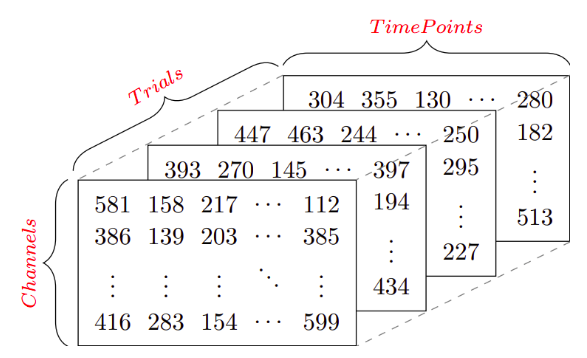
\includegraphics[scale=0.6]{{{ImagesSSVEP/epoch_matrix}.png}}
    \caption{Οι τρεις από τις διαστάσεις του τετραδιάστατου πίνακα όπου αποθηκεύουμε τα σήματα μετά την κατάτμηση. Η τέταρτη διάσταση είναι οι διαφορετικές συχνότητες διέγερσης.}
    \label{fig:epoch_matrix}
\end{figure}

\subsubsection{Preprocessing Pipeline}

\par Η προεπεξεργασία των εγκεφαλικών σημάτων είναι ένα απαραίτητο στάδιο, το οποίο μπορεί να καθορίσει σε μεγάλο ποσοστό την επιτυχία και τα αποτελέσματα του πειράματος. Υπάρχουν αρκετοί λόγοι που καθιστούν την προεπεξεργασία αυτή απαραίτητη. Αρχικά όπως αναφέραμε και στην ενότητα \ref{sec:eeg_intro}, το EEG παρουσιάζει χαμηλή χωρική ανάλυση, με αποτέλεσμα τα σήματα που ανιχνεύονται από τον εγκεφαλογράφο να διαφέρουν σημαντικά συγκριτικά με αυτά τα οποία παρήχθησαν από τον εγκέφαλο. Επιπλέον τα σήματα αυτά, παρουσιάζουν χαμηλό σηματο-θορυβικό λόγο (SNR), με αποτέλεσμα να καλύπτονται σημαντικές αδύναμες συνιστώσες του, που μπορεί να μας ενδιαφέρουν. Σημαντικά είναι και τα παράσιτα (artifacts) λόγω μυικών κινήσεων, όπως η κίνηση των ματιών, ενώ δεν είναι σπάνιο πολλές φορές να μολύνεται το σήμα και από τυχαία εγκεφαλική δραστηριότητα κατά την διάρκεια της καταγραφής.

\par Εδώ θα περιγραφούν τα βήματα που απαιτούνται για το φιλτράρισμα και την ετοιμασία των δεδομένων για την περαιτέρω ανάλυση των σημάτων. Τα βήματα αυτά διαφέρουν από έρευνα σε έρευνα, και όσον αφορά το ποιόν τους αλλά και την σειρά εφαρμογής τους, ανάλογα με τον σκοπό της εργασίας, και γίνεται μια προσπάθεια να οριστεί μια καθολική διαδικασία προ-επεξεργασίας, την οποία θα ακολουθούν όλοι, προκειμένου να είναι και πιο εφικτή η σύγκριση μεταξύ των αποτελεσμάτων από διάφορες εργασίες. Στην διεθνή βιβλιογραφία, το σύνολο αυτών των διαδοχικών διαδικασιών αναφέρεται και ως eeg pipelining. Ένα pipeline που ακολουθείται από πολλούς ερευνητές, περιγράφεται από τον ψυχολόγο Makoto Miyakoshi \cite{noauthor_undated-vj}.

\par Τα κύρια στάδια του pipeline που συνήθως δεν λείπουν από καμία εργασία είναι τα εξής:\\
\begin{itemize}
    \item{Χρήση φίλτρου notch για την αφαίρεση πολύ συγκεκριμένων συχνοτήτων όπως θορύβου τροφοδοσίας (50Hz η 60Hz)}
    \item{Φιλτράρισμα βαθυπερατό-υψηπερατό για απόρριψή DC σημάτων και μη χρήσιμων συχνοτήτων}
    \item{Αφαίρεση artifacts λόγω κινήσεων των ματιών και του κεφαλιού θεωρώντας πως τα artifacts και το σήμα ενδιαφέροντος παράγονται από ξεχωριστές πηγές, και εφαρμόζοντας τεχνικές διαχώρισης πηγών (source seperation) όπως ICA}
    \item{Διάφορες τεχνικές χωρικού φιλτραρίσματος όπως averaging, rereference κ.α}
\end{itemize}

\par Σημαντικό ρόλο παίζει η σειρά με την οποία εφαρμόζουμε καθεμία από τις διαδικασίες του pipeling, 
καθώς είναι γεγονός πως για τις  μη γραμμικές διαδικασίες δεν ισχύει η αντιμεταθετική ιδιότητα, και δίνουν διαφορετικά αποτελέσματα, αναλόγως με την σειρά κατά την οποία θα εφαρμοστούν στο σήμα.

\par Στην παρούσα εργασία, οι συχνότητες ενδιαφέροντος κυμαίνονταν μεταξύ $6Hz$ και $40Hz$, δηλαδή στο διάστημα που ορίζουν οι συχνότητες διέγερσης για τα οπτικά σήματα, και οι αρμονικές τους. Συνεπώς κάνοντας χρήση δύο IIR Butterworth φίλτρων, βαθυπερατό με συχνότητα αποκοπής στα $45Hz$, και υψηπερατό στα $4Hz$, επιτυγχάνουμε την αφαίρεση της DC συνιστώσας του σήματος, και επίσης δεν απαιτείται η χρησιμοποίηση ειδικού φίλτρου για το φιλτράρισμα του θορύβου του ηλεκτρικού ρεύματος τροφοδοσίας. Επιπλέον, απομακρύνεται ένα μεγάλο μέρος των σημάτων που ευθύνονται στην μυική λειτουργία (EMG) (υψίσυχνος θόρυβος), αλλά και σημάτων EOG λόγω της κίνησης των οφθαλμών \cite{Oikonomou2016-ew}. Τέλος ακολουθώντας τις πρακτικές που περιγράφονται στο βιβλίο \cite{Luck2014-mg}, προτιμήθηκε η διαδοχική χρήση βαθυπερατού και υψηπερατού φίλτρου, αντί ενός βαθυπερατού, καθώς και η αφαίρεση της μέσης τιμής του κάθε epoch, πριν και μετά το φιλτράρισμα.

\begin{figure}[H]
    \centering     
    \subfigure[]{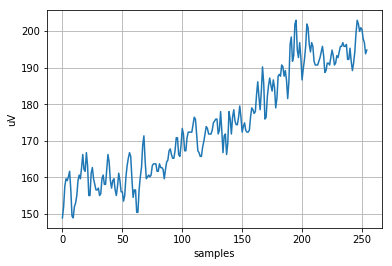
\includegraphics[scale=0.5]{{{ImagesSSVEP/unfiltered}.png}}}
    \subfigure[]{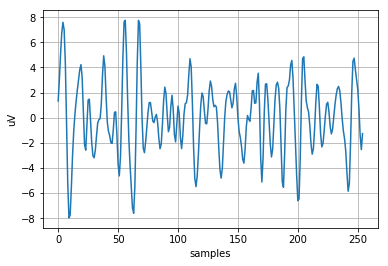
\includegraphics[scale=0.5]{{{ImagesSSVEP/filtered}.png}}}
    \caption{Ένα εγκεφαλικό σήμα διάρκειας 2sec α) πριν και β) μετά την εφαρμογή του φίλτρου}
    \label{fig:filt_before_after}
\end{figure}

\par Όσον αφορά το EPOC συγκεκριμένα, πολλές φορες παρατηρήσαμε πως για κάποιο φαινομενικά ανεξήγητο λόγο σε εμάς, εμφανιζόντουσαν απότομες διακυμάνσεις (spikes) στο σήμα, που δεν δικαιολογούνταν από καμιά εξωτερική η εγκεφαλική επίδραση, πράγμα το οποίο διαπιστώθηκε και στην διπλωματική εργασία \cite{artemis} που χρησιμοποίησε τον ίδιο εγκεφαλογράφο και πιθανώς να προέρχονται από κάποια δυσλειτουργία των ηλεκτρονικών του εγκεφαλογράφου. Υπάρχουν διάφορες τεχνικές εξάλειψης αυτών των epoch που περιέχουν spikes, όπως απόρριψή κάνοντας οπτική επιθεώρηση (rejecting by visual inspection). Εμείς προκειμένου να αυτοματοποιηθεί η διαδικασία, χρησιμοποιήσαμε ένα κατώφλι απόρριψης για το πλάτος του σήματος, διαδικασία που κατατάσσεται στα μη γραμμικά στάδια του pipeline.

\begin{figure}[H]
    \centering     
    \subfigure[]{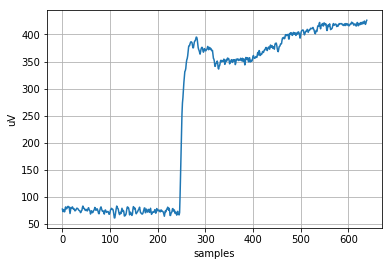
\includegraphics[scale=0.5]{{{ImagesSSVEP/unfiltered_peak_O2}.png}}}
    \subfigure[]{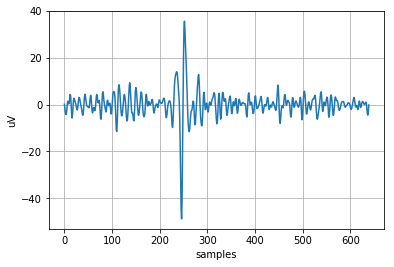
\includegraphics[scale=0.5]{{{ImagesSSVEP/filtered_peak_O2}.png}}}
    \subfigure[]{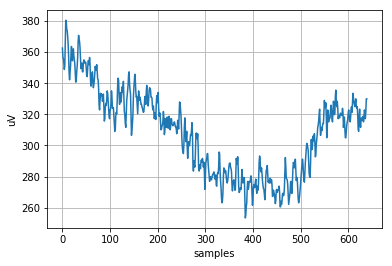
\includegraphics[scale=0.5]{{{ImagesSSVEP/unfiltered_peak_O1}.png}}}
    \subfigure[]{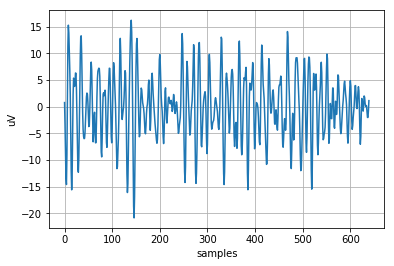
\includegraphics[scale=0.5]{{{ImagesSSVEP/filtered_peak_O1}.png}}}
    \caption{a) Εμφάνιση spike στο κανάλι O2 και b) το σήμα του O2 μετά την εφαρμογή φιλτραρίσματος Για την ίδια χρονική στιγμή παρατηρούμε πως δεν εμφανίζεται spike στο γειτονικό κανάλι O1 c). συνεπώς το spike δεν μπορεί να ευθύνεται σε κάποια κίνηση, η δυνατό τράνταγμα.}
    \label{fig:spikes}
\end{figure}

\par Παρά τις παραπάνω διαδικασίες, συνήθως υπάρχει ακόμα παρών θόρυβος στις συχνότητες 0-10Hz, κυρίως λόγω της κίνησης των βλεφάρων. Η πιο συνήθης τεχνική απομάκρυνσης αυτού του θορύβου, είναι η ανάλυση κυρίων συνιστωσών (ICA), η οποία υποθέτει πως το παραγόμενο σήμα είναι το αποτέλεσμα του γραμμικού συνδυασμού πολλών πηγών (όσων και των διαφορετικών καναλιών-αισθητήρων), μίας εκ των οποίων θα είναι και η κίνηση των βλεφάρων. Αποφασίστηκε να μην χρησιμοποιηθεί αυτή η τεχνική για δύο λόγους. Αρχικά, για να δώσει καλά αποτελέσματα, απαιτεί σήματα μεγάλης διάρκειας, η οποία αυξάνεται εκθετικά καθώς αυξάνονται τα κανάλια. Είναι πολύ ευαίσθητη μέθοδος όσον αφορά την επεξεργασία δεδομένων από διαφορετικές καταγραφές, ακόμα και αν οι συνθήκες των πειραμάτων είναι σχεδόν ίδιες. Για παράδειγμα, έστω πως παρέχουμε στην ICA ένα ικανό αριθμό δεδομένων για να βρει τον κατάλληλο πίνακα μετασχηματισμού των αρχικών καναλιών, στα νέα "κύρια" κανάλια. Αν τον ίδιο πίνακα τον χρησιμοποιήσουμε για τον μετασχηματισμό νέων δεδομένων από τον ίδιο χρήστη, με τον ίδιο εγκεφαλογράφο, αλλά με λίγο διαφορετική τοποθέτηση των ηλεκτροδίων, η ακόμα και αν απλά εφαρμόσουμε λίγο παραπάνω υγρό επαφής, τότε η ICA θα αποτύχει να διαχωρίσει σωστά τα κανάλια \cite{noauthor_undated-vj}. Πράγμα το οποίο συμβαίνει κατά κόρον με εγκεφαλογράφους που δεν επιτρέπουν την ακριβή τοποθέτηση των ηλεκτροδίων στον κρανίο (όπως ο EPOC). Ο δεύτερος λόγος είναι πως στην περίπτωση μας δεν παρατηρήθηκαν έντονα παράσιτα κίνησης των βλεφάρων, καθώς τα ηλεκτρόδια που χρησιμοποιήσαμε βρίσκονται στο πίσω μέρος του εγκεφάλου, τα οποία "μολύνονται" λιγότερο από αυτόν τον μυικό θόρυβο.

\textbf{Σημαντική Παρατήρηση}
\par Μια σημαντική παράμετρος είναι η σειρά με την οποία θα γίνει το pipelining και το epoching. Ένας λόγος για να προτιμήσει κάποιος να γίνουν οι διαδικασίες του pipelining πριν το epoching (πράγμα που συμβαίνει στην πλειοψηφία των περιπτώσεων), είναι το γεγονός πως η εφαρμογή κυρίως των υψιπερατών φίλτρων σε σήματα διάρκειας λίγων δευτερολέπτων, προκαλεί παραμορφώσεις στα άκρα τους (filtering edge artifacts) \cite{noauthor_undated-rl}\cite{Luck2014-mg}. Σε αυτή την εργασία όμως θα κάνουμε το αντίθετο για τον εξής λόγο. Ο απώτερος σκοπός της offline ανάλυσης είναι η εύρεση της καλύτερης μεθόδου έτσι ώστε να χρησιμοποιηθεί στην online εκδοχή της διεπαφής. Όπως γίνεται αντιληπτό, σ' αυτήν την περίπτωση δεν θα έχουμε πρόσβαση στο συνολικό εγκεφαλικό σήμα, παρά μόνο σε παράθυρα λίγων δευτερολέπτων τα οποία αντιστοιχούν στα epochs της offline ανάλυσης. Συνεπώς τα στάδια του pipeline έγιναν μετά την κατάτμηση του συνολικού σήματος, σε κάθε epoch ξεχωριστά, έτσι ώστε να προσομοιώνεται καλύτερα η real-time (online) λειτουργία.

\subsection{Εξαγωγή Χαρακτηριστικών και Συστήματα Απόφασης}
\label{subsec:featureExtract}
\par Πλέον, έχοντας στα χέρια μας τα δεδομένα, φιλτραρισμένα, και ταξινομημένα ανά χρήστη και session, και οργανωμένα σε πίνακες με βάση το κάθε κανάλι, δοκιμή (trial) και συχνότητα οπτικής διέγερσης, εφαρμόζουμε τους αλγορίθμους που περιγράφηκαν στο ενότητα \ref{sec:chap3_feature}, προκειμένου να αξιολογηθούν ως προς την ικανότητα χρήσης τους στην online διεπαφή που θα παρουσιαστεί στην συνέχεια.

\section{Μέθοδοι Φασματικής Ανάλυσης}
\subsection{Ορισμός Μαθηματικής Σημειογραφίας}
\par Προκειμένου να είναι πιο κατανοητές οι τεχνικές που θα περιγραφούν, και να μην υπάρχουν τυχόν παρερμηνείες, ορίζουμε εδώ τις μεταβλητές όπως ορίζονται και μέσα στον κώδικα που υλοποιήθηκε. Αρχικά θεωρούμε ένα BCI σύστημα $N_f$ οπτικών διεγέρσεων, με συχνότητες $f_{stimuli} = [f_1,...,f_{N_f}] \epsilon \mathbb{R}^{N_f}$, και συμβολίζουμε ως $i$ τον δείκτη αυτών των συχνότήτων, με $i = 1,...,N_f$. Συνεπώς έχουμε και $N_f$ πιθανές κλάσεις $c_i$ που αντιστοιχούν στις $f_i$. Έπειτα από την διαδικασία του epoching, προκύπτουν συνολικά $N_t$ trials για κάθε $f_i$ συχνότητα, και ορίζουμε το $t = 1,...,N_t$ ως δείκτη των trials. Ως αποτέλεσμα, συνολικά έχουμε $N_{ep} = N_t\cdot N_f$ epochs. Κάθε ένα από αυτά τα epochs, $epoch_n$, με $n=1,...,N_{ep}$, μπορεί να ανήκει σε μία από τις κλάσεις $c_i$, δηλαδή $C(epoch_n) = c_i$. Η φασματική πυκνότητα του $epoch_n$ συμβολίζεται $PSD(epoch_n)$, και οι $Ν_k$ συχνότητες με την ισχυρότερη παρουσία στο φάσμα δημιουργούν τον διάνυσμα $F_{peaks_{n}} = [F_1,...,F_{N_k}] \epsilon \mathbb{R}^{N_k}$, και με $mag(F_k)], \  k = [1,...,N_k]$ το πλάτος ενός συγκεκριμένου peak στο φάσμα. Τέλος, σε κάποιες από τις ακόλουθες μεθόδους, θα λαμβάνουμε υπόψην μας και τους $N_h$ αρμονικούς μιας $f_i$ συχνότητας, και θα τους συμβολίζουμε ως $h\cdot f_i$, με $h=1,...,N_h$.

\subsection{PSD}
\par Όπως είναι αναμενόμενο, σε κάθε πρόβλημα του οποίου στόχος είναι η ανίχνευση της παρουσίας και της ισχύος συγκεκριμένων συχνοτήτων σε ένα σήμα, τις πιο πολλές φορές εφαρμόζονται τεχνικές που βασίζονται στον μετασχηματισμό Fourier. Δεδομένης της περιγραφής και του τρόπου λειτουργίας των SSVEP σημάτων, θα περίμενε κάποιος πως η συχνότητα της οπτικής διέγερσης, ξεχωρίζει σημαντικά από της υπόλοιπες. Σε αυτή την περίπτωση, μια πρώτη προσέγγιση είναι η εύρεση της συχνότητας $f_{max}=F_{peaks}[1]=F_1$ με την μέγιστη ισχύ για το epoch $epoch_n$, και η ανάθεση του δείγματος, στην κλάση $c_i$ της συχνότητας διέγερσης $f_i$ που βρίσκεται σε μικρότερη απόσταση από την $f_{max}$. Δηλαδή,
\begin{align}%\large
    C(epoch_n) = c_i, \ \  i=\argmin_{i} \Vert f_{max}-f_i \Vert ^2
\end{align}
\par Σε πολλές περιπτώσεις όμως, η επικρατούσα συχνότητα του σήματος, δεν συμπίπτει με την συχνότητα της οπτικής διέγερσης (εικόνα \ref{fig:7Hz8HzGmm}, καθώς όπως έχει αναφερθεί, το σήμα μπορεί να περιλαμβάνει peaks τα οποία να προκύπτουν από άλλες εγκεφαλικές λειτουργίες, ή και από SSVEP σήματα που προκαλούνται από γειτονικές οπτικές διεγέρσεις. Τέλος με αυτό τον τρόπο δεν λαμβάνονται υπόψιν καθόλου οι αρμονικές της συχνότητας διέγερσης που εμφανίζονται στα SSVEP σήματα. Ως αποτέλεσμα, όπως θα φανεί και στο κεφάλαιο των αποτελεσμάτων, ο παραπάνω αλγόριθμος παρουσιάζει χαμηλό ποσοστό επιτυχίας.
\begin{figure}[H]
    \centering     
    \subfigure[]{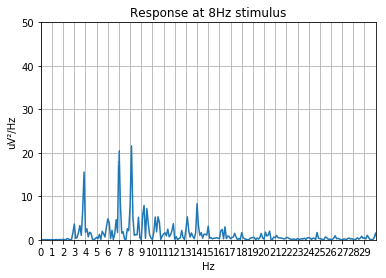
\includegraphics[scale=0.6]{{{ImagesSSVEP/7Hz_for_gmm}.png}}} %[0,:,12,1]
    \subfigure[]{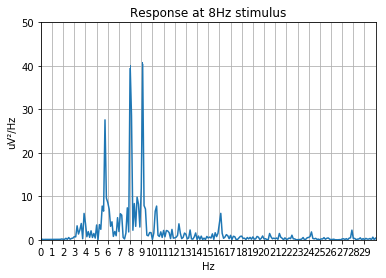
\includegraphics[scale=0.6]{{{ImagesSSVEP/8Hz_for_gmm}.png}}}
    \caption{SSVEP σήματα στο κανάλι Ο1 για ΕΟΔ 7Hz (a) και 8Hz (b). Παρατηρούμε πως και στις δύο περιπτώσεις, η επικρατούσα συχνότητα δεν συμπίπτει με αυτήν της κάθε ΕΟΔ, οπότε ο απλός PSD αλγόριθμος θα έδινε λάθος αποτελέσματα. Ωστόσο, μπορούμε να συμπεράνουμε εύκολα σε ποια ΕΟΔ αντιστοιχεί κάθε σήμα, αν προσέξουμε τα peaks στις πρώτες αρμονικούς (14Hz και 16Hz).}
    \label{fig:7Hz8HzGmm}
\end{figure}

\subsection{PSD - Gaussian Mixture Filtering}
\par Μια λύση που προτείνουμε, είναι η χρήση παραπάνω από μιας επικρατούσας συχνότητας (multiple peaks), σε συνδυασμό με την εφαρμογή μια τεχνικής φιλτραρίσματος των $k$ peaks, κάνοντας χρήση μιας μίξης γκαουσιανών συναρτήσεων για κάθε συχνότητα διέγερσης, με μέσες τιμές τις ίδιες τις συχνότητες διέγερσης και τις αρμονικές τους. Συγκεκριμένα, κατασκευάζουμε την γκαουσιανή μίξη $Gm_i$ για κάθε συχνότητα $f_i$, λαμβάνοντας υπόψιν μας τους $N_h$ πρώτους αρμονικούς της. 
\begin{align}%\large
    Gm_i(f)=\sum_{h=1}^{N_h}a_{ih}\cdot \frac{1}{\sigma_{ih} \sqrt{2 \pi}}\exp(-\frac{(f-h\cdot f_i)^2}{2 \sigma_{ih}^2})
\end{align}

\par Ο συντελεστής διασποράς $\sigma_{ih}$ καθορίζει το εύρος της γκαουσιανής "καμπάνας" για τον $h\text{-στο}$ αρμονικό της συχνότητας $f_i$, ενώ ο $a_{ih}$, το πλάτος της κάθε μίας, και είναι μεταβλητές που παίζουν καθοριστικό ρόλο στην επιτυχία του αλγορίθμου, γι αυτό θα γίνει προσεχτική βελτιστοποίηση τους. 

\par Στην συνέχεια για κάθε $epoch_n$ πολλαπλασιάζουμε το διάνυσμα $F_{peaks_n}$ με κάθε μία από τις $Gm_i$, και προκύπτει το $score_i$ για κάθε μία από τις κατηγορίες $c_i$, δηλαδή,
\begin{align}
    score_i=\sum_{l=1}^{l=3} mag(F_l)\cdot Gm_i(F_l) \  , i =1,...,N
\end{align}
\par Η τελική απόφαση για την κλάση στην οποία ανήκει το δείγμα γίνεται επιλέγοντας αυτή με το μέγιστο score,
\begin{align}
    C(epoch_n) = c_i, \ \ i=\argmax_i(score_i)
\end{align}
\begin{figure}[H]
    \centering     %%% not \center
    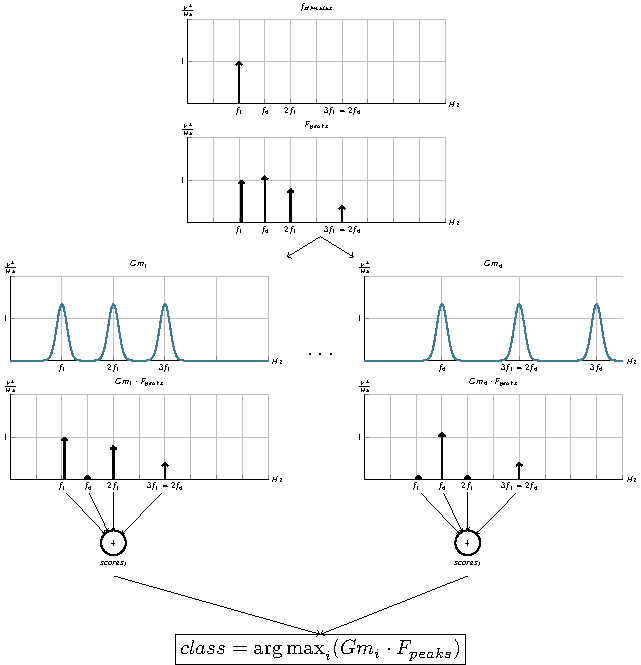
\includegraphics[scale=1.5]{{{LatexDiagrams/GMM___diagram}.pdf}}
    \caption{Σχηματικό παράδειγμα λειτουργίας του αλγορίθμου PSD-GM. Έστω τέσσερις πηγές οπτικής διέγερσης με αντίστοιχες συχνότητες $f_1,f_2,f_3,f_4$. Έστω οτι ο χρήστης κοιτάζει την $f_1$, τότε παράγεται SSVEP σήμα, με επικρατούσες συχνότητες την $f_1$, τις δύο αρμονικές $2f_1,3f_i$ καθώς και την μέγιστη απ' όλες $f_4$. Η κάθε $Gm_i$ αναθέτει υψηλά σκόρ στην $f_i$ και τις αρμονικές της, ενώ παράλληλα σχεδόν μηδενίζει τις υπόλοιπες. Με αυτό τον τρόπο τελικά η $f_1$ θα έχει το μεγαλύτερο score, λόγω της παρουσίας των αρμονικών της στο φάσμα.}
    \label{fig:gmm}
\end{figure}

\subsection{Μέθοδοι βασισμένοι στην CCA}
\par Τα χαρακτηριστικά της μεθόδου, και το τι προσπαθεί να πετύχει εξηγήθηκαν αναλυτικά στην παράγραφο \ref{subsec:cca_theory}, ενώ το ιστορικό εφαρμογής της στα SSVEP σήματα, στο κεφάλαιο \ref{chap:survey} 

\par Στην συγκεκριμένη εφαρμογή, εφαρμόζουμε την CCA έτσι ώστε να βρούμε τον μεγιστο συντελεστή κανονικής συσχέτισης μεταξύ του πίνακα δεδομένων ενός $epoch_n$, $X_n \epsilon \mathbb{R}^{N_c\times N_s}$ και ενός πίνακα $Y_i \epsilon \mathbb{R}^{2N_h\times N_s}$ με ημιτονικά templates της συχνότητας $f_i$,

\begin{align}
\label{eq:cca_templates_Y}
    Y_i = \begin{bmatrix}
            \sin{2\pi f_i t} \\
            \cos{2\pi f_i t} \\
            \vdots \\
            \sin{2\pi N_hf_i t} \\
            \cos{2\pi N_hf_i t} \\
          \end{bmatrix}
          \ \ \ ,
          %\LARGE
    t = \begin{bmatrix}
            \frac{1}{f_s} & \frac{2}{f_s} & \cdots & \frac{N_f}{f_s}
        \end{bmatrix}
\end{align}

\par Ο πίνακας $Y_i$, περιέχει τα σήματα που θα θέλαμε ιδανικά να παράγονται από τον εγκέφαλο ως απόκριση στην οπτική διέγερση $f_i$, συνεπώς, διαισθητικά, ο CCA προσπαθεί να μετασχηματίσει γραμμικά τους δύο πίνακες και να βρει με ποιόν $Y_i$ μοιάζει περισσότερο ο $X_n$, και ορίζει ως μέτρο ομοιότητας (score) την μέγιστη κανονική συσχέτιση. Η παραπάνω διαδικασία εφαρμόζεται $N_f$ φορές, όσες δηλαδή και οι κλάσεις-συχνότητες που έχουμε.
\begin{align}
    CCAscore_i = \rho(X_n^Ta,Y_i^Tb)
\end{align}
\par Όσον αφορά την τελική ανάθεση του epoch σε μια από τις $c_i$ κλάσεις, μπορούμε να ακολουθήσουμε δύο μεθόδους. Αρχικά μπορούμε να το αναθέσουμε στην κλάση της οποίας ο πίνακας $Y_i$ είχε την μεγαλύτερη συσχέτιση με τον $X_n$, δηλαδή,
\begin{align}
    C(epoch_n) = c_i, \ \  i=\argmax_i(CCAscore_i)
    \label{eqCCAmax}
\end{align}
\par Ένας άλλος τρόπος είναι να χρησιμοποιήσουμε τα $N_f$ scores που θα προκύψουν για κάθε $epoch_n$, ως ένα διάνυσμα χαρακτηριστικών, και να γίνει η χρήση ενός αλγορίθμου μηχανικής μάθησης όπως ο kNN. Το διάνυσμα χαρακτηριστικών για κάθε epoch θα είναι, 
\begin{align}
    CCAfeature_n = [CCAscore_1,CCAscore_2,...,CCAscore_{N_f}]
    \label{eqCCAkNN}
\end{align}

\begin{figure}[H]
    \centering     %%% not \center
    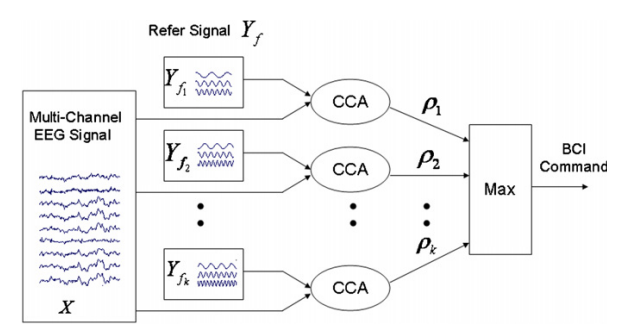
\includegraphics[scale=0.8]{{{ImagesSSVEP/cca_bci}.png}}
    \caption{Σχηματικό παράδειγμα της εφαρμογής του CCA για την αναγνώριση της κλάσης που ανήκει ένα epoch ($X$). Η τελική απόφαση γίνεται με το κριτήριο του μεγίστου που περιγράφεται από την εξίσωση \eqref{eqCCAmax}. Εικόνα από \cite{Bin2009-lt}
    }
    \label{fig:cca}
\end{figure}
%\cite{Nakanishi2015-md} cca survey
\subsection{Συνδυαστική μέθοδος PSD - PCA - MLR - kNN}

\par Στην εργασία \cite{Wang2016-nc}, προτάθηκε μια συνδυαστική μέθοδος που επιτυγχάνει ποσοστά επιτυχίας ανώτερα των μεθόδων PSD, CCA καθώς και κάποιων παραλαγών της CCA (CCA-variants), και περιλαμβάνει τα εξής στάδια. Αρχικά για κάθε $epoch_n$ δημιουργούμε το μονοδιάστατο διάνυσμα $X_n \epsilon \mathbb{R}^N_c\cdot N_p$ που αποτελείται από όλα τα $N_c$ κανάλια σε σειρά (concatenated), με σκοπό να κατασκευαστεί ο πίνακας $X = [X_1, X_2, \cdots, X_{N_{ep}}]$ διαστάσεων $N_c\cdot N_p\times N_{ep}$. Στην συνέχεια εφαρμόζεται PCA για την ελάττωση της διάστασης, επιλέγοντας τις κύριες συνιστώσες μέγιστης διασποράς. Το αποτέλεσμα είναι ένας πίνακας $X_{pca}$ διαστάσεων $N_{pc}\times N_{ep}$, όπου $N_{pc}$ ο αριθμός των κύριων συνιστωσών-χαρακτηριστικών που διατηρήθηκαν. Κατόπιν, κατασκευάζοντας τον πίνακα ετικετών (labels) $Υ$ σύμφωνα με την εξίσωση \eqref{eqMLR1}, εφαρμόζουμε γραμμική παλινδρόμηση MLR για να εξάγουμε τον πίνακα χαρακτηριστικών $X_{mlr}$ διαστάσεων $N_f\times N_{ep}$. Τέλος, τα στοιχεία του $X_{mlr}$ μαζί με τον $Y$ θα χρησιμοποιηθούν ως μοντέλο δεδομένων για έναν kNN αλγόριθμο. 

\par Προκειμένου τώρα ένα καινούριο test δεδομένο να ταξινομηθεί, θα πρέπει να υποστεί τις ίδιες διαδικασίες PCA, και MLR. Συνεπώς, θα πρέπει να αποθηκεύονται οι πίνακες μετασχηματισμού PCA (εξίσωση \eqref{eq2}) και MLR (εξίσωση \eqref{eqMLR2}).

\par Παρότι στην σχετική εργασία, για την δημιουργία του $X_n$ χρησιμοποιήθηκαν τα χρονικά σήματα κάθε καναλιού, σε δοκιμές που κάναμε, δεν μπορέσαμε να αναπαράγουμε τα ίδια θετικά αποτελέσματα. Αντιθέτως, τα ποσοστά επιτυχίας αυξήθηκαν σημαντικά όταν αντί για τα σήματα στον χρόνο, χρησιμοποιήθηκαν οι μετασχηματισμοί τους στο χώρο της συχνότητας (PSD).
\begin{figure}[H]
    \centering     %%% not \center
    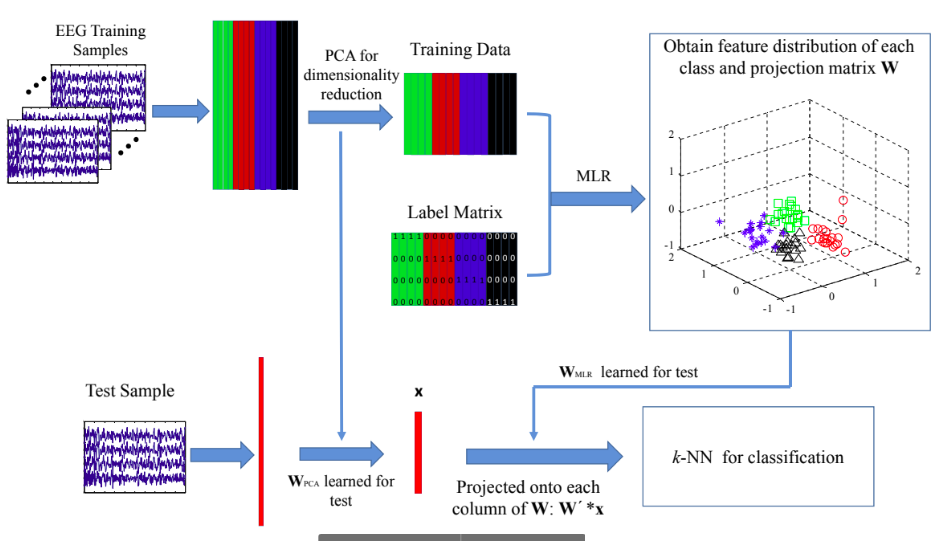
\includegraphics[scale=0.4]{{{ImagesSSVEP/pca-mlr-knn}.png}}
    \caption{Σχηματικό παράδειγμα της συνδιαστικής μεθόδου PCA-MLR-kNN. Η μόνη διαφορά με την μέθοδο που ακολουθήσαμε είναι πως χρησιμοποιήσαμε τα PSD σήματα για κάθε epoch, αντί των χρονικών σημάτων που φαίνονται στο σχήμα. Εικόνα από \cite{Wang2016-nc}
    }
    \label{fig:pca-mlr-knn}
\end{figure}

\subsection{Παρατήρηση για την κατάσταση No-Control (NC)}
\label{subsec:NC}
\par Όπως αναφέρθηκε στην υποενότητα \ref{subsec:protocol}, στο προτόκολο offline καταγραφής, συμπεριλάβαμε και την εντολή NC, έτσι ώστε να εκπαιδεύσουμε το σύστημα μας να αναγνωρίζει τις περιόδους όπου ο χρήστης δεν θέλει να το χρησιμοποιήσει (idle periods). Προκειμένου να το πετύχουμε αυτό, ακολουθήσαμε τις εξής τακτικές. 

\par Όσον αφορά τις μεθόδους που βασίζονται στον kNN, (CCA-kNN και PSD-PCA-MLR-kNN), δεν χρειαζόταν κάποια διαφορετική αντιμετώπιση για τα NC σήματα. Θα γίνεται κανονικά εξαγωγή χαρακτηριστικών (είτε CCA, είτε PSD-PCA-MLR), και την ταξινόμηση τους θα την αναλάβει ο kNN, ο οποίος θα τα αντιμετωπίζει σαν μια ξεχωριστή κλάση.

\par Αντίθετα, για τις υπόλοιπες μεθόδους (PSD-GM, CCA), ακολουθήσαμε μια διαφορετική κατεύθυνση. Τροποποιήσαμε αυτές τις μεθόδους, έτσι ώστε πέρα από το αποτέλεσμα της ταξινόμησης, να επιστρέφουν και ένα δείκτη $confidence$, δηλαδή έναν δείκτη του κατά πόσο είναι σίγουροι για την επιλογή τους. Με αυτό τον τρόπο φτάνει να βρούμε ένα κατάλληλο κατώφλι $Thr_{NC}$ για κάθε διαφορετικό αλγόριθμο, έτσι ώστε να αποφανθούμε για το αν το σήμα ήταν IC η NC. Πιο συγκεκριμένα, όπως είδαμε, και ο PSD-GM αλλά και ο CCA, για την ταξινόμηση ενός σήματος, δίνουν ένα score για κάθε μία από τις τέσσερις κλάσεις (π.χ στην περίπτωση της CCA, την πρώτη κανονική συσχέτιση), τα οποία score στην συνέχεια, είδαμε πως χρησιμοποιούνται ως είσοδος  σε μια συνάρτηση μεγίστου. Συνεπώς ορίσαμε το confidence ως εξής: Έστω ο $x$ αλγόριθμος, όπου αναθέτει ένα δείγμα $s$, με μέγιστο score $score_1$ στην κατηγορία $c_1$, και με αμέσως μικρότερο score $score_2$ στην $c_2$, τότε ορίζουμε,
\begin{align}
    Conf_{X_s} = \frac{score_1 - score_2}{score_1}, \ \ score_i\geqslant 0
\end{align}

Η μέγιστη τιμή για το confidence είναι 1, ενώ η ελάχιστη είναι 0, και αυτό συμβαίνει μόνο στην σπάνια περίπτωση που έχουμε δύο ίδια score, δηλαδή ο αλγόριθμος να ταξινομεί το σήμα, εξίσου, σε δύο διαφορετικές κατηγορίες. 
\par Γενικά, όταν ο χρήστης δεν έχει στραμμένο το βλέμμα του προς κάποια ΕΟΔ, δεν σημαίνει πως στο εγκεφαλικό του σήμα δεν θα εμφανίζονται peaks στις αντίστοιχες συχνότητες. Οποιοδήποτε σημείο και να κοιτάξει, θα "αναβοσβήνει" σε αυτές τις συχνότητες λόγω οπτικών αντανακλάσεων. Ωστόσο περιμένουμε πως στο παραγόμενο σήμα δεν θα ξεχωρίζει κάποια από τις συχνότητες τόσο όσο στην περίπτωση που ο χρήστης κοιτούσε μια από τις ΕΟΔ, συνεπώς, ιδανικά, ο δείκτης confidence θα προσεγγίζει το 0.

\section{Online BCI διεπαφή}
\label{sec:online_design}

\subsection{Περιγραφή Συστήματος}
\par Η online BCI διεπαφή που υλοποιήσαμε χαρακτηρίζεται ως ασύγχρονη \ref{item:asynchronous}, καθώς ο χρήστης ελέγχει το πότε θα κοιτάξει κάποια οπτική διέγερση, χωρίς να του το υπαγορεύει το σύστημα. Η υλοποίηση έγινε δημιουργώντας  threads-agents οι οποίοι επιτελούν διαφορετικές λειτουργίες και ανταλλάσσουν δεδομένα μεταξύ τους μέσω δομών που ονομάζονται "ουρές" (message queue). Συγκεκριμένα τους agents αποτελούν ο Reader(), που που διαβάζει τα πακέτα δεδομένων από το EPOC, ο Plotter(), που όταν είναι ενεργοποιημένος εμφανίζει την γραφική διεπαφή για την οπτικοποίηση των σημάτων, ο Classifier() ο οποίος είναι υπεύθυνος για την υλοποίηση των αλγορίθμων ταξινόμησης που υλοποιήθηκαν στην προηγούμενη ενότητα, και ο Commander() ο οποίος λαμβάνει το αποτέλεσμα της ταξινόμησης και το μετασχηματίζει σε χρήσιμες εντολές για την εκτέλεση μιας διαδικασίας όπως η κίνηση του δείκτη του ποντικιού, το πάτημα συγκεκριμένων πλήκτρων. Όσον αφορά την διαδικασία, δημιουργήθηκε o MazeApp(), ο οποίος υλοποιεί ένα παιχνίδι λαβυρίνθου, στο οποίο ο χρήστης πρέπει να μετακινήσει τον χαρακτήρα του προς τον στόχο, χρησιμοποιώντας τις κατάλληλες εντολές. Τέλος, η Memory δεν είναι τίποτα άλλο, παρά μια ουρά Last In First Out, η οποία καταχωρεί το ιστορικό των εντολών που πάρθηκαν.
\begin{figure}[H]
    \centering     %%% not \center
    \subfigure[]{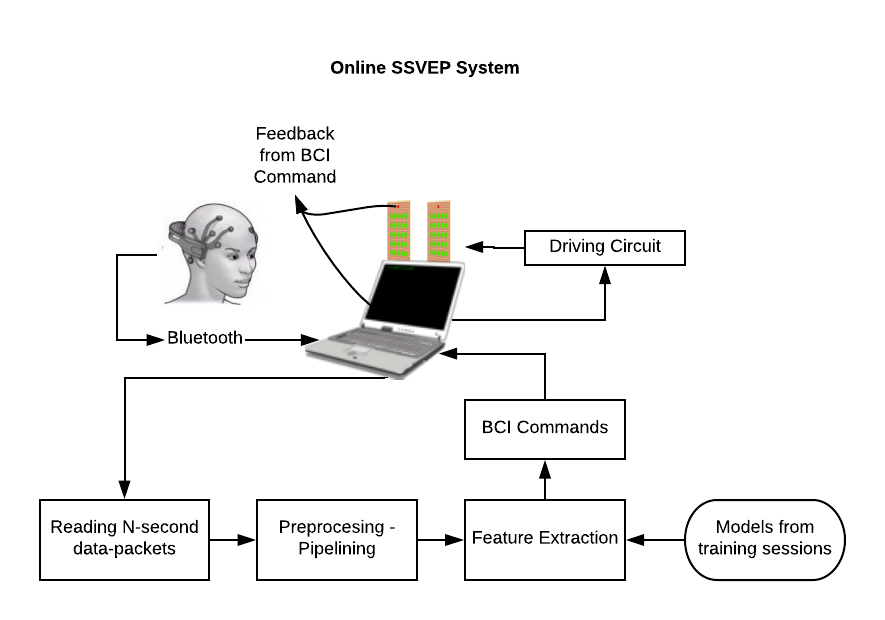
\includegraphics[scale=0.4]{{{ImagesSSVEP/online}.png}}}
    \subfigure[]{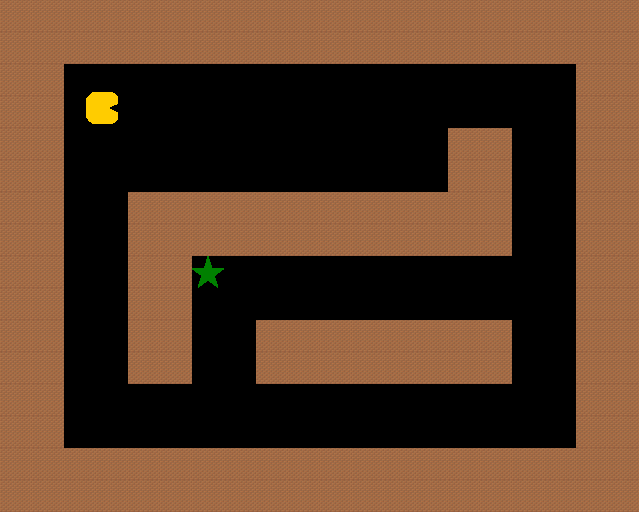
\includegraphics[scale=0.3]{{{ImagesSSVEP/task_game}.png}}}
    \caption{a) Το γενικό διάγραμμα λειτουργίας της οnline BCI διεπαφής, b) το απλό παιχνίδι λαβυρίνθου στο οποίο ο χρήστης έπρεπε να κατευθύνει το avatar του (pacman) πρoς το πράσινο άστρο. }
    \label{fig:online_uml_maze}
\end{figure}


\par Το avatar μπορεί να κινηθεί ελεύθερα και προς τις τέσσερις δυνατές κατευθύνσεις, συνεπώς αντιστοιχίζουμε καθεμία από τις οπτικές διεγέρσεις, σε μια κατεύθυνση. Επιπλέον προσθέσαμε μια ακόμα εντολή, της οποίας η λειτουργία είναι να αναιρεί την προηγούμενη εντολή που πάρθηκε. Καθώς όμως δεν είχαμε πέμπτη ΕΟΔ για να αντιστοιχήσουμε αυτή την εντολή, χρησιμοποιήσαμε την ανίχνευση άλφα κυμάτων. Επιλέχθηκαν τα άλφα κύματα επειδή είναι κύματα τα οποία μπορούν να παραχθούν πολύ εύκολα από την πλειοψηφία των χρηστών, κλείνοντας απλά τα μάτια τους, και επίσης είναι σχετικά εύκολη η αναγνώρισή τους. Μια σκέψη είναι πως η ανίχνευση τους μπορεί να πραγματοποιηθεί από τους αλγορίθμους που περιγράψαμε για τα SSVEP σήματα, καθώς μπορούμε να θεωρήσουμε πως είναι SSVEP σήματα που προκλήθηκαν από μια ΕΟΔ συχνότητας $10-11Hz$. Ένας άλλος απλούστερος τρόπος, ο οποίος έδωσε και καλύτερα αποτελέσματα, είναι η μέτρηση της συνολικής ενέργειας στην ζώνη 10-12Hz, και ο ορισμός ενός κατωφλιού $Alpha_{thr}$, πάνω από το οποίο θα θεωρούμε πως ο χρήστης έχει κλειστά τα μάτια του. Και με τους δύο τρόπους θα πρέπει να γνωρίζουμε εκ των προτέρων είτε την άλφα συχνότητα κάθε χρήστη, είτε την μέση ισχύ των άλφα κυμάτων του, πράγμα το οποίο απαιτεί ένα επιπλέον στάδιο (calibration stage) κατά την online λειτουργία.

\par Μια άλλη παράμετρος η οποία πρέπει να ρυθμιστεί είναι το πόσο συχνά λαμβάνεται απόφαση από το σύστημα, το οποίο καθορίζεται από το μέγεθος του παραθύρου το οποίο θα επεξεργαζόμαστε και το οποίο αντιστοιχεί στην διάρκεια του κάθε epoch της offline ανάλυσης. Η επιλογή χρονικού παραθύρου επηρεάζει την ακρίβεια του αλγορίθμου, καθώς και τον $ITR$, που αποτελεί συνάρτηση αυτών των δύο. Η εύρεση ισορροπίας μεταξύ $A_c$ και $ITR$ εξαρτάται από τον στόχο που έχει θέσει κάθε έρευνα, όπως θίξαμε και στο κεφάλαιο \ref{chap:survey}.

\par Τέλος, μπορούμε να ελέγξουμε την συχνότητα των λανθασμένων εντολών (misclassification rate) ρυθμίζοντας τον Classifier(), να στέλνει την τελική εντολή, μόνο όταν αυτή εμφανιστεί $k$ συνεχόμενες φορές. Επιπλέον μπορούμε να ελέγξουμε τον ρυθμό των NC false positives, ρυθμίζοντας ανάλογα το κατώφλι $NC_{thr}$. Όσο μεγαλύτερες αυτές οι δύο τιμές, τόσο μεγαλύτερη θα είναι η ακρίβεια, αλλά και τόσο περισσότερο θα καθυστερεί να πάρει απόφαση το σύστημα.\\

\begin{figure}[H]
    \centering     %%% not \center
    \subfigure[]{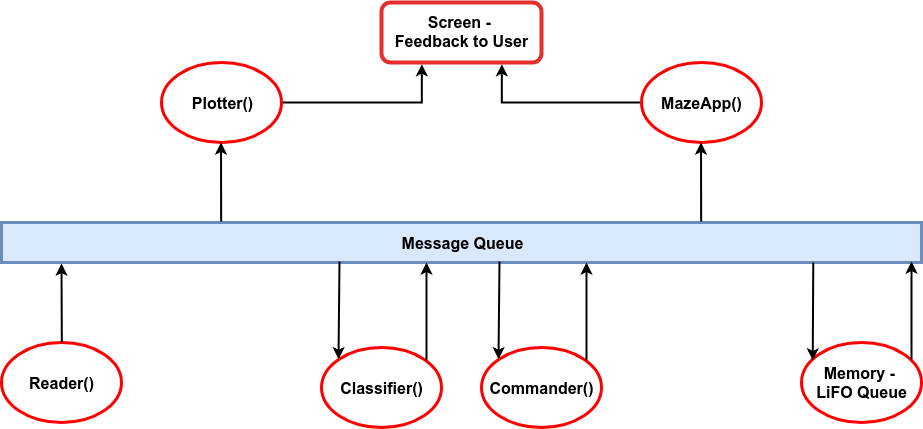
\includegraphics[scale=0.4]{{{ImagesSSVEP/online_uml}.png}}}
    \subfigure[]{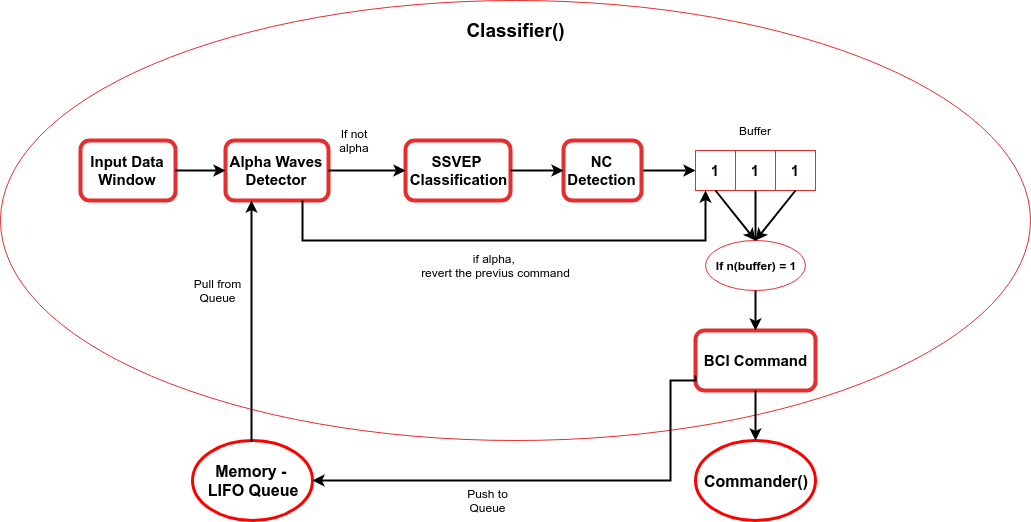
\includegraphics[scale=0.4]{{{ImagesSSVEP/classifier_uml}.png}}}
    \caption{a) Το διάγραμμα λειτουργίας των threads-agents που αποτελούν την online διεπαφή, και b) Το διάγραμα λειτουργίας του agent Classifier(), και η σχέση του με την Memory η οποία κρατάει ιστορικό των προηγούμενων εντολών, και τον Commander() που παίρνει το αποτέλεσμα της ταξινόμησης και το μετατρέπει σε εντολή. Συμβολίζουμε με $n(\cdot )$ το πλήθος των μοναδικών στοιχείων ενός συνόλου.}
    \label{fig:online_umls}
\end{figure}

\end{document}
